\documentclass[11pt,a4paper]{ctexart}
% Shared preamble for the assignment reports. Use with:
%   \documentclass[11pt,a4paper]{ctexart}  (XeLaTeX)
%   % Shared preamble for the assignment reports. Use with:
%   \documentclass[11pt,a4paper]{ctexart}  (XeLaTeX)
%   % Shared preamble for the assignment reports. Use with:
%   \documentclass[11pt,a4paper]{ctexart}  (XeLaTeX)
%   \input{../common/preamble.tex}
\usepackage[margin=2.3cm]{geometry}
\setmainfont{texgyretermes}[Extension=.otf,UprightFont=*-regular,BoldFont=*-bold,ItalicFont=*-italic,BoldItalicFont=*-bolditalic]
\setsansfont{texgyreheros}[Extension=.otf,UprightFont=*-regular,BoldFont=*-bold,ItalicFont=*-italic,BoldItalicFont=*-bolditalic]
\setmonofont{texgyrecursor}[Extension=.otf,UprightFont=*-regular,BoldFont=*-bold,ItalicFont=*-italic,BoldItalicFont=*-bolditalic]
\usepackage{amsmath,amssymb,mathtools,bm}
\usepackage{graphicx}
\usepackage{booktabs,multirow,makecell,array,tabularx}
\usepackage[table]{xcolor}
\usepackage[most]{tcolorbox}
\usepackage{enumitem}
\usepackage{listings}
\usepackage{subcaption}
\usepackage{siunitx}
\usepackage[hidelinks]{hyperref}
\usepackage[nameinlink,noabbrev]{cleveref}
\usepackage{float}

\setlength{\emergencystretch}{3em}
\linespread{1.15}
\setlist{leftmargin=*,itemsep=2pt,topsep=3pt}
\graphicspath{{figures/}}

\crefname{figure}{图}{图}
\crefname{table}{表}{表}
\crefname{section}{第}{第}
\creflabelformat{section}{#2#1#3 节}
\crefname{equation}{式}{式}
\crefformat{equation}{式~(#2#1#3)}

\lstset{basicstyle=\ttfamily\footnotesize,columns=fullflexible,breaklines=true,frame=single,
  framerule=0.3pt,rulecolor=\color{black!40},backgroundcolor=\color{black!3},
  keywordstyle=\color{blue!60!black}\bfseries,commentstyle=\color{green!40!black},
  numbers=left,numberstyle=\tiny\color{black!50},xleftmargin=1.5em}

% Interview boxes: question, model answer, common wrong answer.
\newtcolorbox{iqbox}[1]{enhanced,breakable,colback=blue!3,colframe=blue!45!black,boxrule=0.5pt,arc=1.5pt,
  left=4pt,right=4pt,top=3pt,bottom=3pt,fonttitle=\bfseries\small,title={面试追问：#1}}
\newtcolorbox{findingbox}[1][]{enhanced,breakable,colback=green!3,colframe=green!40!black,boxrule=0.5pt,arc=1.5pt,
  left=4pt,right=4pt,top=3pt,bottom=3pt,fonttitle=\bfseries\small,title={结论#1}}
\newtcolorbox{caveatbox}{enhanced,breakable,colback=orange!4,colframe=orange!60!black,boxrule=0.5pt,arc=1.5pt,
  left=4pt,right=4pt,top=3pt,bottom=3pt,fonttitle=\bfseries\small,title={不能推出的结论}}

\newcommand{\authorline}{ShaneLiu04\thanks{GitHub: \url{https://github.com/ShaneLiu04}。代码与原始指标：\url{https://gitee.com/liu-xingyan04/mlsys-infra}。本文基于公开课程材料独立完成，与课程团队无隶属关系。}}

\usepackage[margin=2.3cm]{geometry}
\setmainfont{texgyretermes}[Extension=.otf,UprightFont=*-regular,BoldFont=*-bold,ItalicFont=*-italic,BoldItalicFont=*-bolditalic]
\setsansfont{texgyreheros}[Extension=.otf,UprightFont=*-regular,BoldFont=*-bold,ItalicFont=*-italic,BoldItalicFont=*-bolditalic]
\setmonofont{texgyrecursor}[Extension=.otf,UprightFont=*-regular,BoldFont=*-bold,ItalicFont=*-italic,BoldItalicFont=*-bolditalic]
\usepackage{amsmath,amssymb,mathtools,bm}
\usepackage{graphicx}
\usepackage{booktabs,multirow,makecell,array,tabularx}
\usepackage[table]{xcolor}
\usepackage[most]{tcolorbox}
\usepackage{enumitem}
\usepackage{listings}
\usepackage{subcaption}
\usepackage{siunitx}
\usepackage[hidelinks]{hyperref}
\usepackage[nameinlink,noabbrev]{cleveref}
\usepackage{float}

\setlength{\emergencystretch}{3em}
\linespread{1.15}
\setlist{leftmargin=*,itemsep=2pt,topsep=3pt}
\graphicspath{{figures/}}

\crefname{figure}{图}{图}
\crefname{table}{表}{表}
\crefname{section}{第}{第}
\creflabelformat{section}{#2#1#3 节}
\crefname{equation}{式}{式}
\crefformat{equation}{式~(#2#1#3)}

\lstset{basicstyle=\ttfamily\footnotesize,columns=fullflexible,breaklines=true,frame=single,
  framerule=0.3pt,rulecolor=\color{black!40},backgroundcolor=\color{black!3},
  keywordstyle=\color{blue!60!black}\bfseries,commentstyle=\color{green!40!black},
  numbers=left,numberstyle=\tiny\color{black!50},xleftmargin=1.5em}

% Interview boxes: question, model answer, common wrong answer.
\newtcolorbox{iqbox}[1]{enhanced,breakable,colback=blue!3,colframe=blue!45!black,boxrule=0.5pt,arc=1.5pt,
  left=4pt,right=4pt,top=3pt,bottom=3pt,fonttitle=\bfseries\small,title={面试追问：#1}}
\newtcolorbox{findingbox}[1][]{enhanced,breakable,colback=green!3,colframe=green!40!black,boxrule=0.5pt,arc=1.5pt,
  left=4pt,right=4pt,top=3pt,bottom=3pt,fonttitle=\bfseries\small,title={结论#1}}
\newtcolorbox{caveatbox}{enhanced,breakable,colback=orange!4,colframe=orange!60!black,boxrule=0.5pt,arc=1.5pt,
  left=4pt,right=4pt,top=3pt,bottom=3pt,fonttitle=\bfseries\small,title={不能推出的结论}}

\newcommand{\authorline}{ShaneLiu04\thanks{GitHub: \url{https://github.com/ShaneLiu04}。代码与原始指标：\url{https://gitee.com/liu-xingyan04/mlsys-infra}。本文基于公开课程材料独立完成，与课程团队无隶属关系。}}

\usepackage[margin=2.3cm]{geometry}
\setmainfont{texgyretermes}[Extension=.otf,UprightFont=*-regular,BoldFont=*-bold,ItalicFont=*-italic,BoldItalicFont=*-bolditalic]
\setsansfont{texgyreheros}[Extension=.otf,UprightFont=*-regular,BoldFont=*-bold,ItalicFont=*-italic,BoldItalicFont=*-bolditalic]
\setmonofont{texgyrecursor}[Extension=.otf,UprightFont=*-regular,BoldFont=*-bold,ItalicFont=*-italic,BoldItalicFont=*-bolditalic]
\usepackage{amsmath,amssymb,mathtools,bm}
\usepackage{graphicx}
\usepackage{booktabs,multirow,makecell,array,tabularx}
\usepackage[table]{xcolor}
\usepackage[most]{tcolorbox}
\usepackage{enumitem}
\usepackage{listings}
\usepackage{subcaption}
\usepackage{siunitx}
\usepackage[hidelinks]{hyperref}
\usepackage[nameinlink,noabbrev]{cleveref}
\usepackage{float}

\setlength{\emergencystretch}{3em}
\linespread{1.15}
\setlist{leftmargin=*,itemsep=2pt,topsep=3pt}
\graphicspath{{figures/}}

\crefname{figure}{图}{图}
\crefname{table}{表}{表}
\crefname{section}{第}{第}
\creflabelformat{section}{#2#1#3 节}
\crefname{equation}{式}{式}
\crefformat{equation}{式~(#2#1#3)}

\lstset{basicstyle=\ttfamily\footnotesize,columns=fullflexible,breaklines=true,frame=single,
  framerule=0.3pt,rulecolor=\color{black!40},backgroundcolor=\color{black!3},
  keywordstyle=\color{blue!60!black}\bfseries,commentstyle=\color{green!40!black},
  numbers=left,numberstyle=\tiny\color{black!50},xleftmargin=1.5em}

% Interview boxes: question, model answer, common wrong answer.
\newtcolorbox{iqbox}[1]{enhanced,breakable,colback=blue!3,colframe=blue!45!black,boxrule=0.5pt,arc=1.5pt,
  left=4pt,right=4pt,top=3pt,bottom=3pt,fonttitle=\bfseries\small,title={面试追问：#1}}
\newtcolorbox{findingbox}[1][]{enhanced,breakable,colback=green!3,colframe=green!40!black,boxrule=0.5pt,arc=1.5pt,
  left=4pt,right=4pt,top=3pt,bottom=3pt,fonttitle=\bfseries\small,title={结论#1}}
\newtcolorbox{caveatbox}{enhanced,breakable,colback=orange!4,colframe=orange!60!black,boxrule=0.5pt,arc=1.5pt,
  left=4pt,right=4pt,top=3pt,bottom=3pt,fonttitle=\bfseries\small,title={不能推出的结论}}

\newcommand{\authorline}{ShaneLiu04\thanks{GitHub: \url{https://github.com/ShaneLiu04}。代码与原始指标：\url{https://gitee.com/liu-xingyan04/mlsys-infra}。本文基于公开课程材料独立完成，与课程团队无隶属关系。}}

\graphicspath{{../../solutions/cmu15849/serving-memory/artifacts/figures/}}

\title{CMU 15-849 推理服务与显存论文复现：\\PagedAttention、iteration-level 调度与 chunked prefill 的模型与 RTX 5090 实测}
\author{\authorline}
\date{2026 年 10 月}

\begin{document}
\maketitle

\begin{abstract}
本报告复现推理服务方向的三篇关键论文——vLLM/PagedAttention~\cite{kwon2023}、Orca 的 iteration-level 调度~\cite{yu2022} 与 Sarathi-Serve 的 chunked prefill~\cite{agrawal2024}。
CPU 部分（已有，20 个测试）实现块管理器（refcount、fork/CoW、swap、recompute 抢占）、KV 显存浪费分析与基于 roofline 的调度模拟器（H100 + Llama-3-8B 参数）。
GPU 部分在一张 RTX 5090 上用自写的 Qwen2.5-0.5B 前向（与 HF transformers 在 fp32 下 logits 最大差 $1.5\times10^{-4}$、argmax 100\% 一致）做三件事：
（1）prefill/decode roofline：decode 在 CUDA graph 下 batch 1 为 2.16 ms/步（462 tok/s），是带宽 roofline 的 3.3 倍——瓶颈是每步约 1000 个小 kernel（按代码逐层计数约 40 个/层），而不是 HBM；
eager 模式每步固定约 8.5 ms，完全由 CPU 下发决定；prefill 在 8192 token 时达到 173.9 TFLOP/s（实测 GEMM 峰值的 73\%）；
（2）Triton 分页 decode attention：块表间接寻址几乎零开销（与连续块表时间相差 $<1\%$），比 PyTorch gather 快 2.2--10.7 倍，比按 4096 预分配的连续缓存 + SDPA 快 3.3--6.9 倍；
4 GiB 预算下真实 GPU 分配，按最大长度预留浪费 86.8\%（并发 85）、分页（block=16）浪费 1.26\%（并发 593），与 lab 模型相差 $\le1.2$ 个百分点；
（3）一个真实的连续批处理引擎（分页 KV + iteration-level 调度 + chunked prefill）在泊松负载下与静态批处理对比：static 饱和于 5.36 req/s（闭式容量模型 5.53），
continuous 在 40 req/s 时 TTFT P99 仍为 38 ms，容量为 static 的 7.5--15 倍；chunked prefill 在 10\% 长 prompt（3072 token）时把逐请求最大卡顿 P99 从 33.5 ms 降到 17.6 ms，
代价是长 prompt 的 TTFT 变为 3.2 倍，lab 的短 prompt 分布下则无收益；引擎迭代时间 $=9.15$ ms $+1.03\times$ roofline，lab 成本模型斜率正确但缺固定开销（\cref{sec:engine,sec:theory-srv}）。
\end{abstract}

\tableofcontents
\newpage

\section{背景与作业要求}
15-849 没有官方编程作业；推理服务方向的论文（vLLM、Sarathi）晚于 2022 年春季课程，但属于该课程“ML 系统”主线的自然延伸，也是推理岗面试的必考点。
我们把论文命题映射为可检验的实验题：

\begin{table}[H]\centering\small
\caption{论文命题与实验对应}
\begin{tabularx}{\linewidth}{>{\raggedright\arraybackslash}p{3.0cm}>{\raggedright\arraybackslash}X>{\raggedright\arraybackslash}X}
\toprule
论文 & 可检验命题 & 本实验 \\
\midrule
vLLM / PagedAttention~\cite{kwon2023} & 连续预留浪费 60--80\%；分页把浪费限制在块尾；块表间接寻址开销小 & CPU 块管理器 + 浪费分析；GPU 上 Triton~\cite{tillet2019} 分页 kernel、真实分配测浪费 \\
Orca~\cite{yu2022} & iteration-level 调度显著提高吞吐、降低排队延迟 & CPU roofline 模拟；GPU 上真实引擎 vs 静态批 \\
Sarathi-Serve~\cite{agrawal2024} & 长 prefill 造成 decode 卡顿（generation stall），chunked prefill 消除之 & 同上，chunk=512 token 预算；测迭代时间线与 inter-token 延迟 \\
Roofline~\cite{williams2009} / LLM 推理分析~\cite{pope2023} & decode 访存受限，batch 增大到拐点前近似免费 & GPU 上 decode 吞吐随 batch/ctx，拐点与模型对照 \\
\bottomrule
\end{tabularx}
\end{table}

GPU 部分按任务说明分三题：B1 用真实模型测 prefill 与 decode 的 roofline、找拐点，并用实测 5090 带宽/算力重算 lab 调度模型（原来用的是 H100 数字）；
B2 最小的分页 KV 注意力（块表 gather）与连续 KV 对比：正确性、随 block 大小的开销、在 lab 的长度分布上实测显存浪费；
B3 一个小型真实连续批处理引擎（泊松到达、变长请求）对比静态批处理：吞吐、TTFT、TPOT、延迟 CDF 随负载，以及 chunked prefill 开/关下的 decode 卡顿。

\section{实验环境}
\begin{table}[H]\centering\small
\caption{软硬件环境（取自 raw 文件的 env 行）}
\begin{tabularx}{\linewidth}{l>{\raggedright\arraybackslash}X}
\toprule
本地 & Windows Server，4 物理核；CPU 部分与绘图在此运行 \\
GPU & NVIDIA GeForce RTX 5090，32 GB GDDR7，170 SM，sm\_120，96 MB L2 \\
软件 & PyTorch 2.8.0+cu128，CUDA 12.8，Triton 3.4.0，Python 3.12.3，transformers（仅用于校验） \\
模型 & Qwen2.5-0.5B（bf16），494,032,768 参数（含 QKV bias），24 层，$d$=896，14 个 query 头 / 2 个 KV 头，head\_dim 64 \\
实测探针 & 512 MiB D2D 拷贝 1518 GB/s；8192$^3$ bf16 GEMM 238.7 TFLOP/s（\texttt{roofline.jsonl}） \\
约束 & 7 个代理共享一卡，GPU 命令在 \texttt{flock} 下串行；CPU 仅 2 核（\texttt{taskset -c 44,45}） \\
\bottomrule
\end{tabularx}
\end{table}
2 个 CPU 核对本文结论有实质影响：eager 模式下 Python 端 kernel 下发是 decode 的瓶颈（\cref{sec:roofline}），引擎的每次迭代也受此限制。这不是缺陷，而是推理系统必须用 CUDA graph、
多步调度、C++ 调度器的原因；报告中对每个数都标注它是 graph 还是 eager 口径。

Qwen2.5-0.5B 每 token 的 KV 为 $2\times24\times2\times64\times2=12{,}288$ 字节（GQA 7:1），是 Llama-3-8B（131,072 字节）的 1/10.7，
所以本文的绝对显存量比 lab 的 H100 模拟小一个数量级，但浪费\emph{比例}与长度分布有关而与模型无关，可直接比较。

\section{方法与实现}
\subsection{CPU 部分（已有）}
\texttt{block\_manager.py}：定长块、块表、refcount、fork + copy-on-write、swap out/in、recompute 抢占，以及按块表 gather 的注意力与逐块 online-softmax 版本（与连续注意力逐位相等）。
\texttt{waste.py}：最大长度预留 / 已知最终长度 / 分页 \{8,16,32,64\} 的生命周期平均浪费与并发数。\texttt{scheduler.py}：static、continuous（Orca）、chunked（Sarathi）三种策略的离散时间模拟，
步时间取 roofline：$\max(\text{FLOPs}/\text{peak},\ (W + \text{KV})/\text{BW})$。\texttt{workload.py}：prompt $\sim$ LogNormal($\ln256$, 1.0) 截断 [8, 3072]，
output $\sim$ LogNormal($\ln128$, 0.9) 截断 [4, 1024]，泊松到达。GPU 部分全部复用这套长度分布与到达过程（相同种子）。

\subsection{GPU：自写 Qwen2 前向}
\texttt{gpu/qwen.py} 从 safetensors 读权重，把 $W_q,W_k,W_v$ 与 gate/up 各自拼成一个 GEMM；前向接受\emph{展平的不规则 token 批}（形状 $[T]$ 的 token 与位置），
attention 是回调，因此同一份权重既可用于连续 KV 的 roofline 测试，也可用于分页 KV 的引擎。

\begin{lstlisting}[language=Python,caption={展平 token 批的前向（gpu/qwen.py，节选）}]
for i, lw in enumerate(self.layers):
    h = self.rms(x, lw["ln1"])
    q, k, v = F.linear(h, lw["wqkv"], lw["bqkv"]).split([H*D, Hk*D, Hk*D], -1)
    q = self.rope(q.view(T, H, D), pos); k = self.rope(k.view(T, Hk, D), pos)
    o = attn(i, q, k, v.view(T, Hk, D))          # 连续 KV / 分页 KV 由回调决定
    x = x + F.linear(o.reshape(T, H*D), lw["wo"])
    gate, up = F.linear(self.rms(x, lw["ln2"]), lw["wgu"]).split(self.ff, -1)
    x = x + F.linear(F.silu(gate) * up, lw["wd"])
\end{lstlisting}

decode 的 GQA 不展开 KV：把同一 KV 头对应的 7 个 query 头折叠到“query 长度”维，\texttt{q.view(B, Hk, 7, D)} 与 \texttt{k[B, Hk, L, D]} 直接做 SDPA，
避免 \texttt{repeat\_interleave} 带来的 7 倍 KV 读放大。

\subsection{GPU：Triton 分页 decode attention}
每个 program 负责一个（序列，query 头），沿块表一次加载 \texttt{PAGES} 个物理块（共 64 个 token 的 tile），用 online softmax 累加：
\begin{lstlisting}[language=Python,caption={分页 decode kernel 主循环（gpu/paged\_attn.py）}]
for p0 in range(0, n_pages, PAGES):
    pg  = p0 + page_of                       # 本 tile 中每个 token 所在的逻辑块
    tok = pg * BLOCK + in_page
    valid = tok < n
    blk = tl.load(BT + b * s_btb + pg, mask=pg < n_pages, other=0)   # 块表查表
    off = blk * s_kb + in_page * s_kt + kvh * s_kh
    k = tl.load(K + off[:, None] + offs_d[None, :], mask=valid[:, None], other=0.).to(tl.float32)
    s = tl.where(valid, tl.sum(k * q[None, :], 1), -float("inf"))
    m_new = tl.maximum(m_i, tl.max(s, 0)); alpha = tl.exp(m_i - m_new); p = tl.exp(s - m_new)
    v = tl.load(V + off[:, None] + offs_d[None, :], mask=valid[:, None], other=0.).to(tl.float32)
    acc = acc * alpha + tl.sum(p[:, None] * v, 0); l_i = l_i * alpha + tl.sum(p, 0); m_i = m_new
\end{lstlisting}
对照实现：\texttt{gather\_decode}（PyTorch 按块表 gather 成 $[B,H_k,L_{\max},D]$ 再带掩码 SDPA）、\texttt{padded\_decode}（连续缓存 $[B,H_k,4096,D]$ 或补齐到批内最长，带掩码 SDPA），
以及同一个 Triton kernel 使用“连续块表”（物理块按序排列），用来分离“间接寻址”本身的代价。正确性以 fp32 逐序列循环为参考。

\subsection{GPU：显存浪费的真实分配}
在 4 GiB 的 KV 预算下，用与 \texttt{waste.py} 相同的 10,000 个请求长度（seed 0），按稳态快照采样：以概率 $\propto$ 输出长度抽取请求（驻留时间正比于输出步数，
与 \texttt{waste.py} 的生命周期平均一致），再在其生成过程中均匀取一个时刻得到在用长度。连续方案为每个序列真实 \texttt{torch.empty} 一块（4096 或最终长度）直到预算用尽；
分页方案分配一个 4 GiB 的池，用 lab 的 \texttt{BlockManager} 发放块。另做一个分配器“搅动”实验：64 个槽位，按最终长度为每个请求分配张量并在完成时释放，共 6000 个请求，
记录 PyTorch 缓存分配器的 reserved/allocated，用来观察 lab 未建模的\emph{外部碎片}。

\subsection{GPU：连续批处理引擎}\label{sec:engine-impl}
\texttt{gpu/engine.py}（约 300 行）是一个真实的单卡服务引擎：
\begin{itemize}
\item \textbf{KV}：一个 $[L,2,\text{num\_blocks},16,H_k,D]$ 的池（2 GiB，10,922 块），按需分配块；新 token 的 KV 用 slot 映射 \texttt{index\_copy\_} 写入；
\item \textbf{每次迭代一次前向}：所有 decode token 与 prefill 块拼成一个展平批，线性层一次算完；decode attention 用 Triton 分页 kernel，prefill 块对“已缓存上下文 + 本块”用带因果偏移掩码的 SDPA；
\item \textbf{策略}：\texttt{static}（凑满一批后左填充到最长 prompt，跑到最长输出结束，已完成成员继续占位）、\texttt{continuous}（Orca/vLLM-v0：每次迭代重组批，新请求整段 prefill，$\le8192$ token）、
\texttt{chunked}（Sarathi：每次迭代 512 token 预算，先 decode，再用剩余预算切 prefill 块）；与 CPU 模拟器的参数一致（max\_num\_seqs=128）。静态批的批大小取连续预留下 2 GiB 能放的序列数（42）；
\item \textbf{时间}：虚拟时钟按每次迭代的实测 wall time 推进（含调度、下发、采样同步），空闲期直接跳到下一个到达，不 sleep；
\item \textbf{抢占}：块不够时抢占最新请求并 recompute（与 CPU 模拟器相同）；本文负载下未触发。
\end{itemize}
continuous 与 chunked 在同一模型上贪心解码得到的 token 完全一致，static 批中最长 prompt 的序列也与之一致（\texttt{tests/test\_gpu\_serving.py} 中的引擎测试；
静态批的左填充未加掩码，只用于计成本，见 \cref{sec:caveat}）。

\subsection{测试}
CPU 侧 20 个测试不变。新增 \texttt{tests/test\_gpu\_serving.py}：块表是物理块的划分、gather 与 fp32 参考一致（CPU）、Triton kernel 在 block=8/16/32/64 下与参考一致
（长度含 1、15、16、17、4096 等边界）、三种调度策略贪心 token 一致（CPU 上用 gather 代替 Triton）。

%==========================================================================
\section{实验结果}

\subsection{CPU：KV 浪费与调度模拟（H100 + Llama-3-8B 模型）}
\begin{figure}[H]\centering
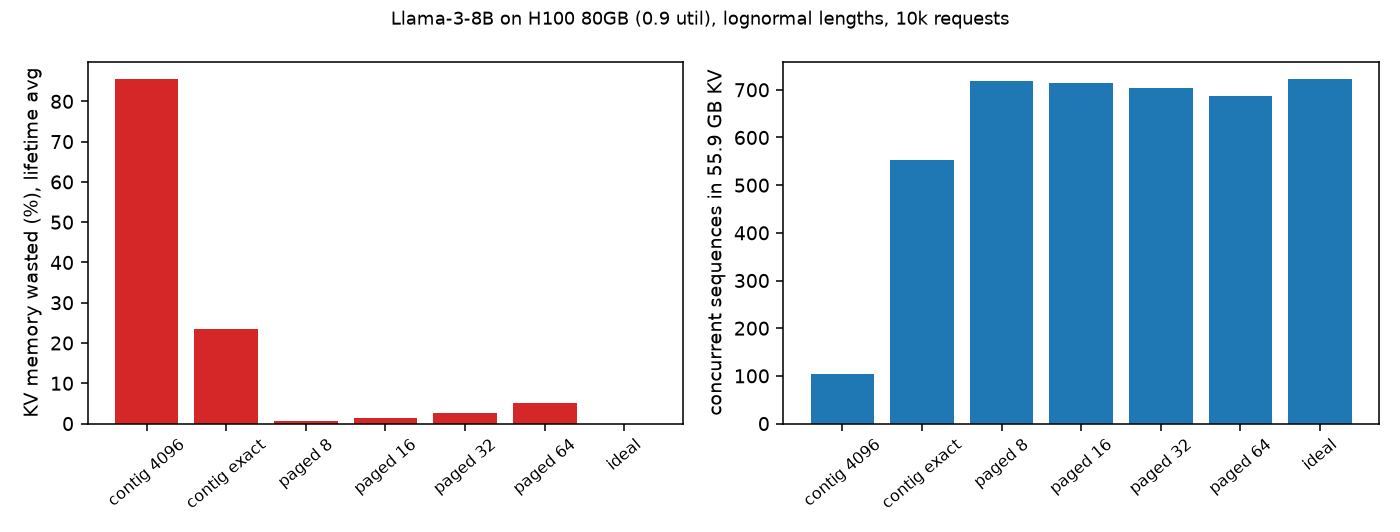
\includegraphics[width=0.8\linewidth]{kv_waste.png}
\caption{10k 请求的生命周期平均 KV 浪费与 80 GB H100 上的并发数（\texttt{kv\_waste.csv}）。}
\label{fig:kvwaste}
\end{figure}
\Cref{fig:kvwaste}：按 4096 连续预留浪费 85.6\%，只能并发 104 条；即使预知最终长度也浪费 23.5\%（生成过程中长度从 prompt 涨到终值）；
分页 block=16 浪费 1.25\%，并发 714 条（6.9 倍）。浪费 $\approx(\text{block}/2)/\bar L$：$8/590\approx1.4\%$。

\begin{figure}[H]\centering
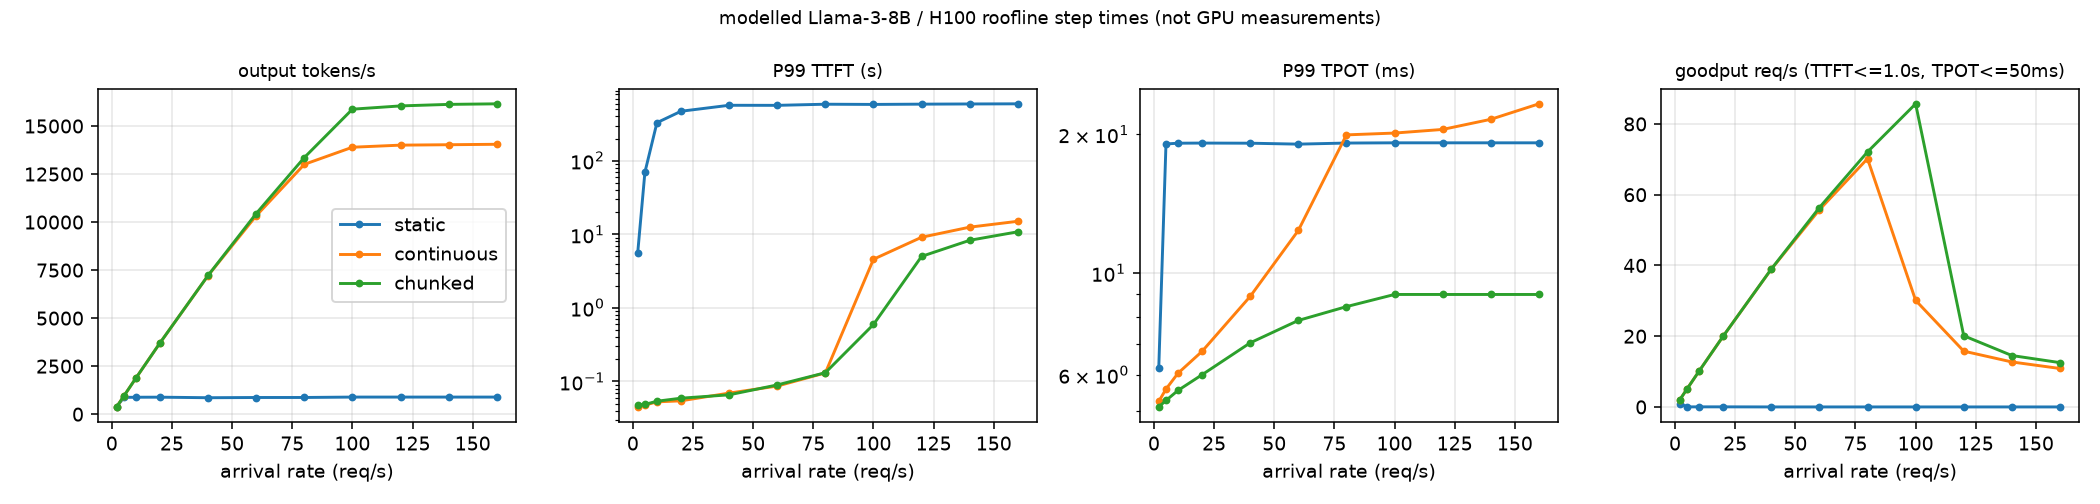
\includegraphics[width=0.85\linewidth]{latency_vs_load.png}
\caption{roofline 调度模拟：吞吐、TTFT、TPOT 随到达率（3000 请求，\texttt{scheduler\_sweep.csv}）。}
\label{fig:simload}
\end{figure}
\Cref{fig:simload}：在“100\% 峰值、零开销”的 H100 模型里，iteration-level 调度把饱和吞吐从 891 提到 14,050 tok/s，chunked prefill 再到 16,156 tok/s，
最长单次迭代从 121 ms 降到 9.2 ms。这些都是模型输出；下面的 GPU 实验检验其中哪些假设成立。

%--------------------------------------------------------------------------
\subsection{GPU B1：prefill 与 decode 的 roofline}\label{sec:roofline}
\begin{figure}[H]\centering
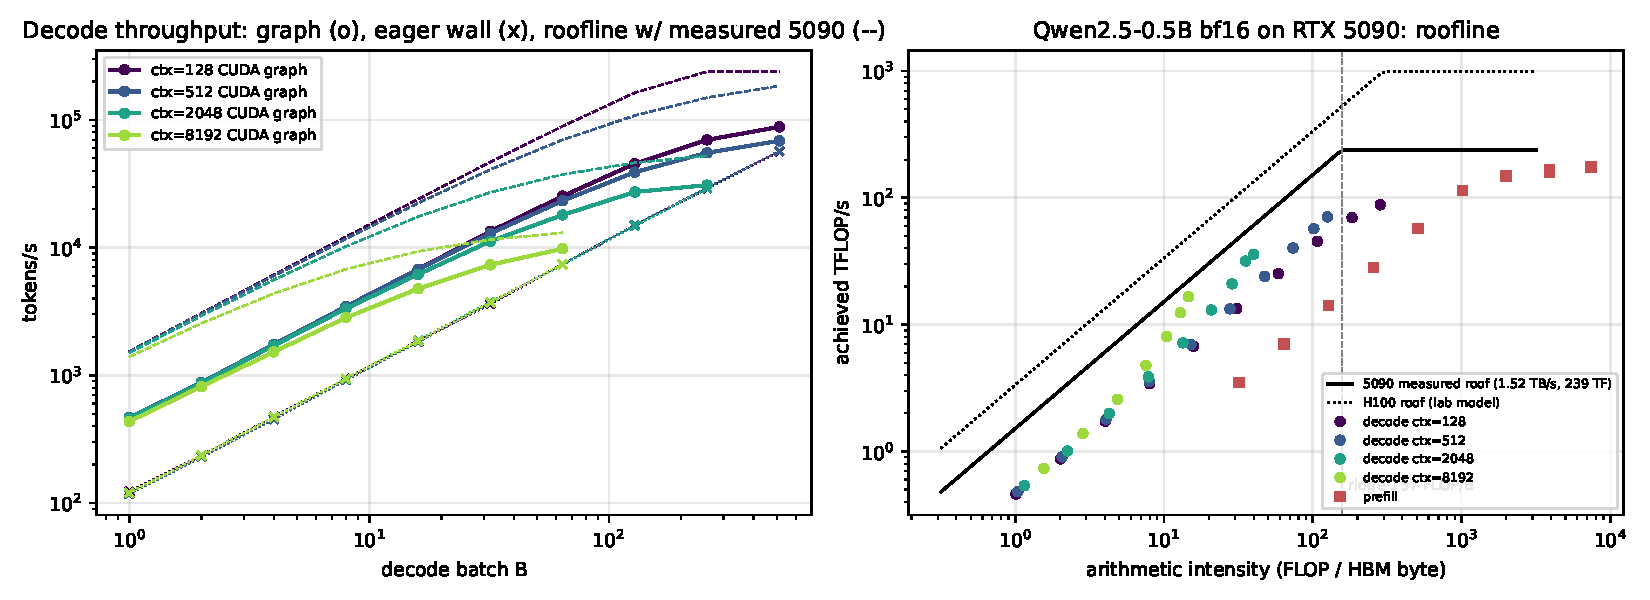
\includegraphics[width=\linewidth]{srv_decode_roofline.pdf}
\caption{左：decode 吞吐随 batch（圆点 CUDA graph，叉号 eager wall time，虚线为用实测 5090 参数的 roofline）；右：roofline 图（decode 圆点、prefill 方块）。}
\label{fig:roof}
\end{figure}
\begin{table}[H]\centering\small
\caption{decode 每步时间（ms，\texttt{roofline.jsonl}；graph = CUDA graph 重放，eager = 每步同步的 wall time）}
\label{tab:decode}
\begin{tabular}{rrrrrrrr}
\toprule
ctx & 口径 & B=1 & B=8 & B=32 & B=64 & B=128 & B=256 \\
\midrule
128 & graph & 2.163 & 2.330 & 2.391 & 2.533 & 2.822 & 3.672 \\
128 & eager & 8.165 & 8.484 & 8.841 & 8.642 & 8.581 & 8.834 \\
512 & graph & 2.145 & 2.314 & 2.482 & 2.752 & 3.285 & 4.633 \\
2048 & graph & 2.168 & 2.405 & 2.857 & 3.554 & 4.698 & 8.300 \\
8192 & graph & 2.300 & 2.834 & 4.369 & 6.534 & — & — \\
\bottomrule
\end{tabular}
\end{table}
\Cref{fig:roof,tab:decode} 给出三个层次的瓶颈：
\begin{enumerate}
\item \textbf{eager：CPU 下发受限。} 不论 batch 是 1 还是 512、上下文是 128 还是 8192，eager 每步都是 8.2--9.0 ms。每步约 1000 次 kernel 下发，在 2 个 CPU 核上每次约 8 µs，
GPU 实际干活远少于此；吞吐因此严格正比于 batch（左图叉号是斜率为 1 的直线），batch 1 只有约 120 tok/s。
\item \textbf{CUDA graph：kernel 数受限。} 用 graph 消除下发后，batch 1 为 2.16 ms（462 tok/s），而带宽 roofline 是 $W/\text{BW}=0.988\,\text{GB}/1.518\,\text{TB/s}=0.65$ ms——
仍差 3.3 倍。原因是约 1000 个 kernel 每个都有 1.5--2.5 µs 的最小执行时间（尾效应、SM 启动），小模型的单层权重只有 30 MB 左右，单个 GEMM 远不足以把 HBM 打满；
实测有效带宽只有 457 GB/s。只有当 KV 读量变大（ctx=8192, B=64：1137 GB/s）时有效带宽才接近 roofline。
\item \textbf{大 batch：计算/小 GEMM 效率受限。} ctx=128 时 B=512 每步 5.81 ms，算术强度 284 FLOP/B 已越过拐点（157 FLOP/B），达到 88k tok/s；
但 $d=896$ 的窄 GEMM 只能跑到约 90 TFLOP/s（GEMM 峰值的 37\%）。
\end{enumerate}

我们把“拐点”定义为步时间相对 B=1 翻倍的最小 batch：ctx = 128/512/2048/8192 时分别为 512/256/128/64。上下文越长，KV 读量越早超过权重读量，拐点越早。
这和 roofline 模型的定性结论一致，但定量上\emph{模型拐点更早}：模型认为 B=1 就已贴着带宽上限，而实际 B 从 1 到 64 几乎免费，因为瓶颈根本不在带宽。

\begin{figure}[H]\centering
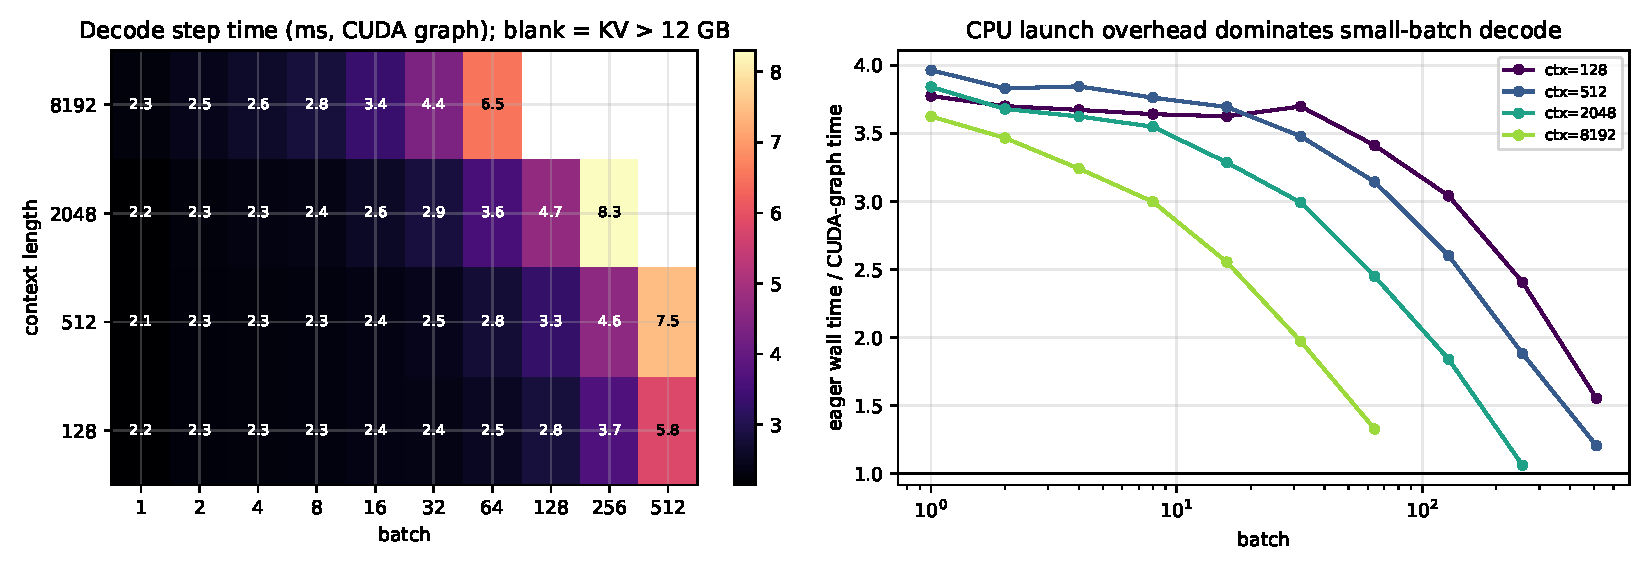
\includegraphics[width=\linewidth]{srv_decode_heatmap_graph.pdf}
\caption{左：decode 步时间热力图（CUDA graph）；右：eager / graph 时间比——小 batch 时 CPU 开销是 GPU 时间的 3.4--3.9 倍。}
\label{fig:heat}
\end{figure}
\Cref{fig:heat} 右图：eager/graph 比在 B=1 时约 3.8，到 ctx=2048、B=256 时降到约 1.06——batch 足够大时 GPU 时间终于盖住 CPU 下发。
推论：在 Python 服务栈里，提高 batch 的第一收益是\emph{摊薄 CPU 开销}，而不是摊薄权重读取；这正是 vLLM 对 decode 默认开 CUDA graph、SGLang/vLLM-v1 把调度挪出关键路径的原因。

\begin{figure}[H]\centering
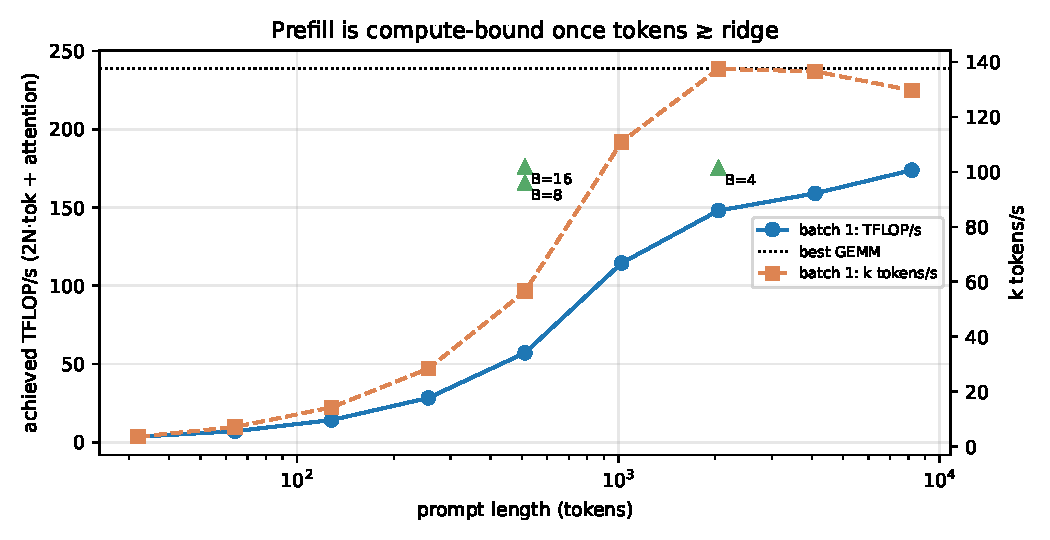
\includegraphics[width=0.8\linewidth]{srv_prefill.pdf}
\caption{prefill 吞吐与算力随 prompt 长度（batch 1；三角为 batch>1）。}
\label{fig:prefill}
\end{figure}
\Cref{fig:prefill}：batch 1 的 prefill 在 $s\le1024$ 时时间恒为 9.0--9.2 ms——又是 eager 下发的平台（此测量未用 graph）；
$s=1024$ 时 111k tok/s、114.5 TFLOP/s；$s=8192$ 时 173.9 TFLOP/s（实测 GEMM 峰值 238.7 的 73\%），tokens/s 从 137.6k（2048）降到 129.7k（8192），
因为注意力的 $O(s^2)$ FLOPs 开始占比。batch 16$\times$512 与 4$\times$2048 都在 175 TFLOP/s 左右。结论：prefill 只要凑够 $\gtrsim$2k token 就是计算受限的，
chunked prefill 的 512 token 块在这张卡上\emph{不能}打满算力（512 token 时 57.1 TFLOP/s），这是 chunk 大小的下界约束。

\begin{figure}[H]\centering
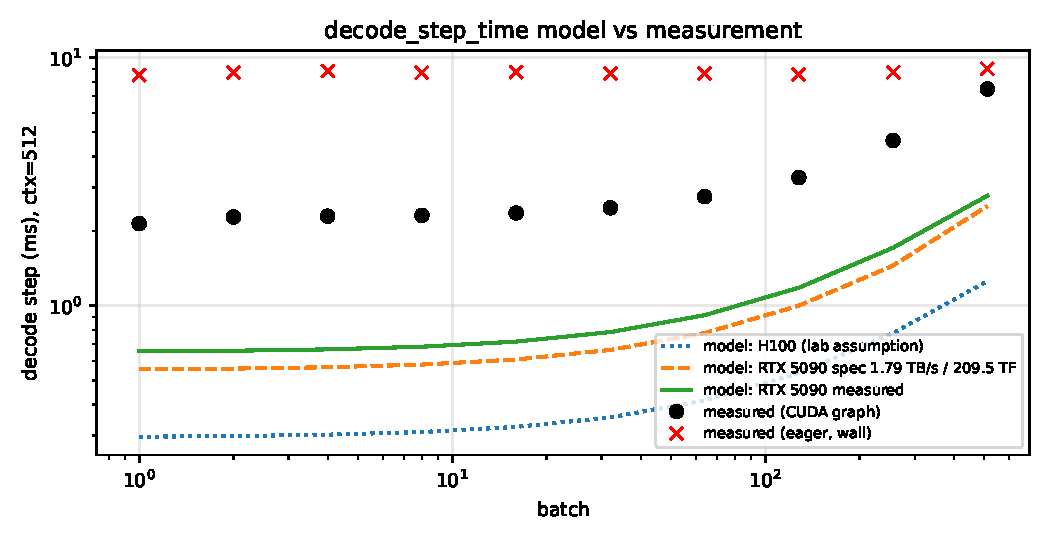
\includegraphics[width=0.75\linewidth]{srv_decode_model_vs_measured.pdf}
\caption{\texttt{mlsys\_calc.decode\_step\_time} 在 H100（lab 假设）、5090 名义、5090 实测参数下的预测 vs 实测（ctx=512）。}
\label{fig:dmodel}
\end{figure}
\Cref{fig:dmodel} 回答“lab 调度模型的假设在 5090 上是否成立”：用 H100 参数（3.35 TB/s）预测会再快 2.2 倍；即使换成实测 5090 参数（1.518 TB/s、238.7 TFLOP/s），
graph 实测仍是模型的 3.28 倍（B=1）到 2.69 倍（B=512）。换言之，lab 模拟器里所有 decode 步时间都应乘以 2.7--3.5（graph）或更多（eager），
它的绝对吞吐是乐观 3 倍以上的下界；但\emph{相对}结论（continuous $\gg$ static、chunked 削平尖峰）不依赖这个系数，\cref{sec:engine} 会验证。

\begin{findingbox}[：roofline]
0.5B 模型 decode 的瓶颈依次是：CPU 下发（eager 8.5 ms/步，与 batch 无关）$\to$ kernel 数（graph 2.2 ms/步，带宽利用 30\%）$\to$ 长上下文时的 KV 带宽或大 batch 时的窄 GEMM 效率。
roofline 只描述最后一层；对小模型直接套 $W/\text{BW}$ 会低估步时间 3 倍以上。
\end{findingbox}

%--------------------------------------------------------------------------
\subsection{GPU B2a：分页 attention 的正确性与开销}
正确性（\texttt{verify.jsonl}）：对 block = 8/16/32/64、两种头配置（Qwen 的 14/2/64 与 Llama-3-8B 的 32/8/128），Triton kernel 与 fp32 逐序列参考的最大绝对误差为
$1.6\times10^{-3}$--$3.4\times10^{-3}$，低于 bf16 的单位舍入 $2^{-8}=3.9\times10^{-3}$；PyTorch gather 版为 $1.6\times10^{-3}$--$3.4\times10^{-3}$，二者同量级——误差来自 bf16 输入与输出舍入，而不是算法。

\begin{figure}[H]\centering
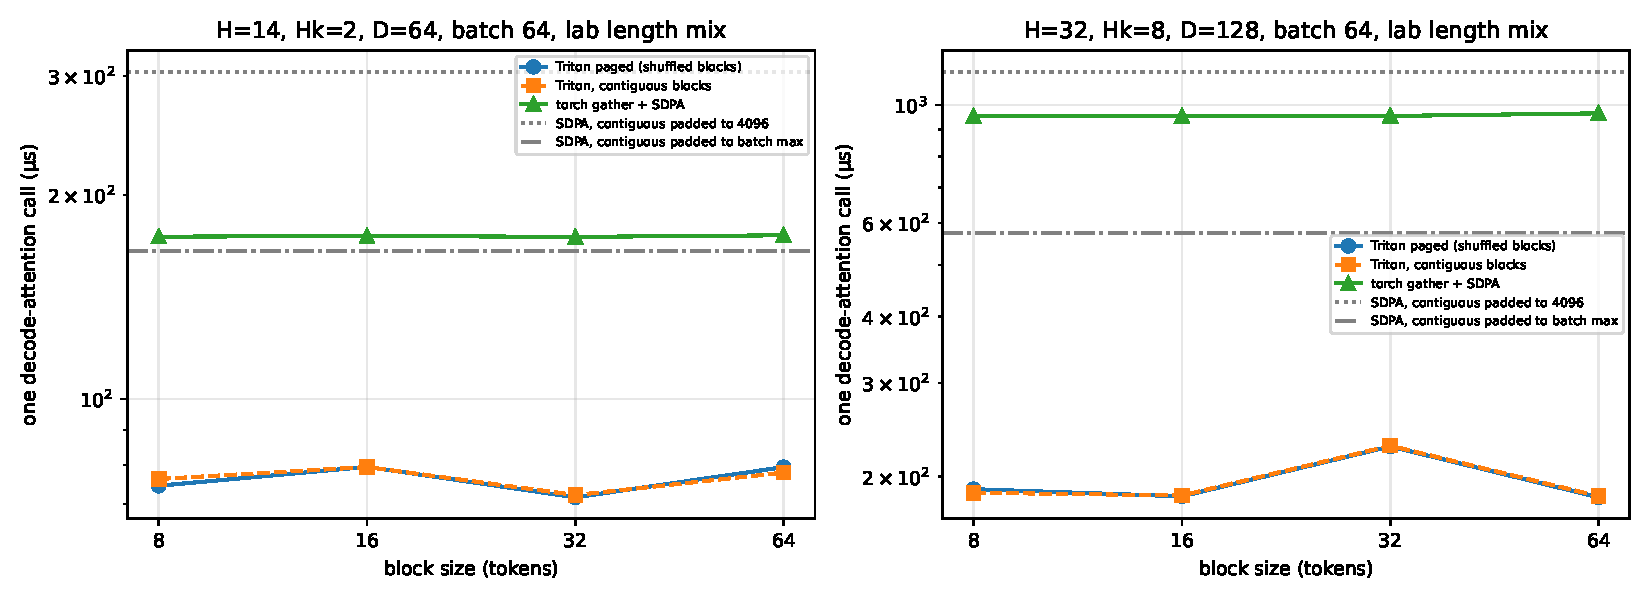
\includegraphics[width=\linewidth]{srv_paged_blocksize.pdf}
\caption{一次 decode attention 调用的时间随 block 大小（batch 64，lab 长度分布在生成中途的快照）。}
\label{fig:pblock}
\end{figure}
\begin{table}[H]\centering\small
\caption{一次 decode attention（µs，block=16，\texttt{paged.jsonl}）；括号内为只计在用 KV 字节的有效带宽 GB/s}
\label{tab:paged}
\begin{tabular}{llrrrrr}
\toprule
头配置 & batch & Triton 分页 & Triton 连续块表 & torch gather & SDPA 补齐批内最长 & SDPA 预留 4096 \\
\midrule
14/2/64 & 16 & 49.6 (62) & 49.6 (62) & 127.6 & 104.1 & 256.2 \\
14/2/64 & 64 & 79.4 (214) & 79.4 (214) & 174.1 & 165.6 & 304.2 \\
14/2/64 & 256 & 165.1 (414) & 165.3 (413) & 713.1 & 448.1 & 536.6 \\
32/8/128 & 16 & 63.0 (388) & 70.4 (347) & 163.9 & 120.5 & 335.8 \\
32/8/128 & 64 & 183.5 (741) & 184.2 (739) & 954.3 & 573.9 & 1155.6 \\
32/8/128 & 256 & 526.1 (1039) & 524.8 (1041) & 5619.7 & 2972.7 & 3632.7 \\
\bottomrule
\end{tabular}
\end{table}
\Cref{fig:pblock,tab:paged} 的要点：
\begin{itemize}
\item \textbf{间接寻址几乎免费}：同一 kernel 用随机打乱的物理块与按序排列的物理块，时间相差 $<1\%$（唯一例外是 32/8/128、batch 16 时分页反而快 11\%，属于调度噪声）。
16 个 token $\times$ 128 维 $\times$ 2 字节 = 4 KB 的块对 DRAM 来说已经是足够大的连续段，随机访问块不会损失带宽。
\item \textbf{block 大小影响很小}：kernel 每次循环固定加载 64 个 token（\texttt{PAGES}$\times$\texttt{BLOCK}），block 8--64 的时间在 $\pm15\%$ 内波动，没有单调趋势。
vLLM 选 16 主要是为了显存浪费（下一节）与块表大小的折中，而不是 kernel 速度。
\item \textbf{gather 是反模式}：PyTorch 先把页 gather 成连续张量再算，多了一次完整的 KV 读写，并且按批内最长补齐，batch 256 时慢 4.3--10.7 倍。
\item \textbf{连续预留的代价不止显存}：预留 4096 的 SDPA 要读整块缓存（掩码不省带宽），比分页慢 3.3--6.9 倍；即使只补齐到批内最长，也慢 1.9--5.7 倍，因为长度分布右偏（P99 prompt 2583）。
\end{itemize}
在 32/8/128、batch 256 时分页 kernel 有效带宽 1039 GB/s，为拷贝带宽的 68\%；14/2/64 时 KV 太小（batch 16 只有 3 MB），一次调用被启动与尾效应主导。

\begin{figure}[H]\centering
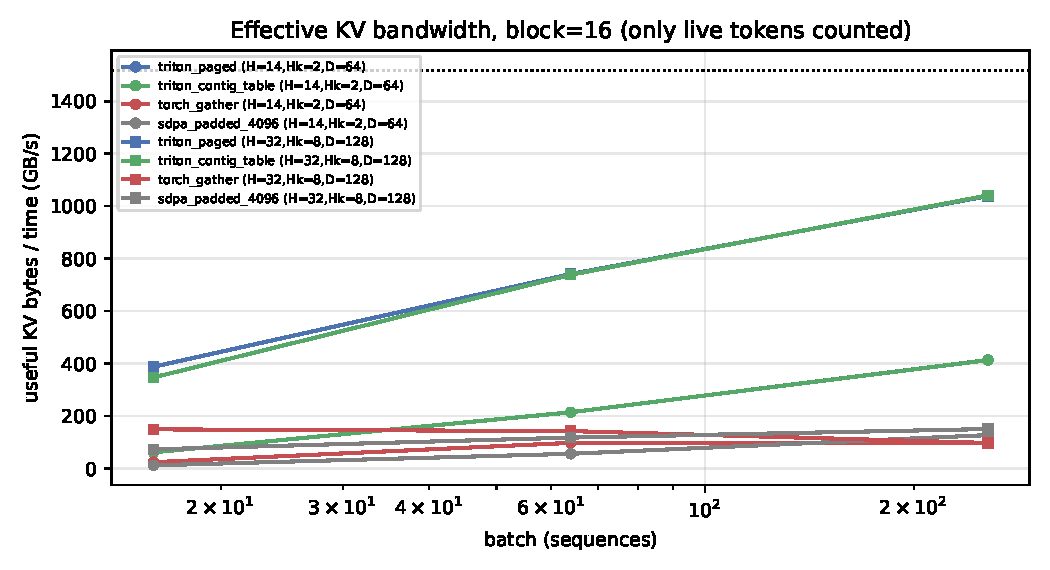
\includegraphics[width=0.78\linewidth]{srv_paged_bandwidth.pdf}
\caption{有效 KV 带宽随 batch（block=16）：分页 kernel 随 batch 增长而逼近 HBM 带宽，gather 与预留 4096 的方案停在 100--150 GB/s。}
\label{fig:pbw}
\end{figure}
\Cref{fig:pbw}：只有分页 kernel 的有效带宽随 batch 单调上升，说明它的工作量正比于在用 token 数；另外两种方案的工作量正比于“分配的” token 数，所以有效带宽被浪费比例压住。
这把“显存浪费”与“带宽浪费”联系起来：连续预留 86.8\% 的浪费（\cref{tab:waste}），在 decode 时同样变成 86.8\% 的无效读（若 kernel 不能按长度提前终止）。

%--------------------------------------------------------------------------
\subsection{GPU B2b：真实分配下的 KV 浪费与外部碎片}\label{sec:waste}
\begin{figure}[H]\centering
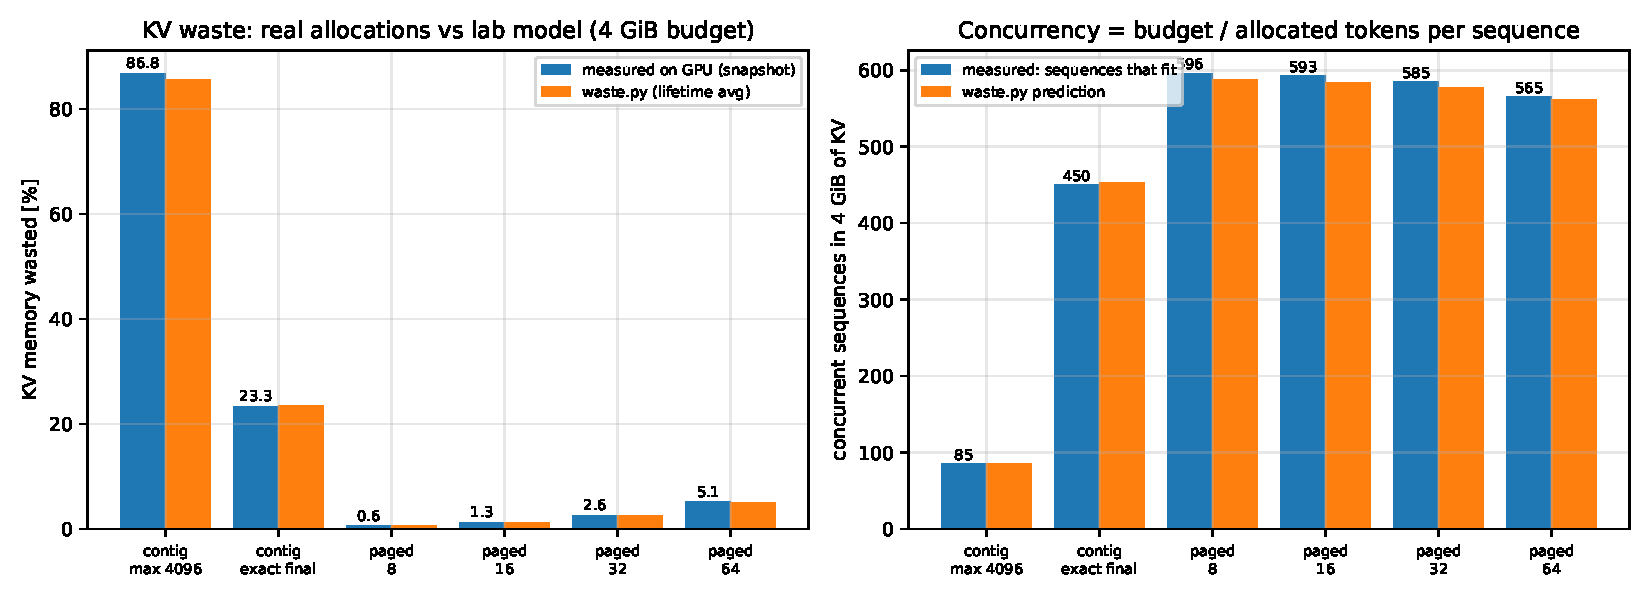
\includegraphics[width=\linewidth]{srv_waste_measured.pdf}
\caption{4 GiB KV 预算下的实测浪费与并发数（蓝）vs \texttt{waste.py}（橙）。}
\label{fig:waste}
\end{figure}
\begin{table}[H]\centering\small
\caption{4 GiB KV 预算下的显存浪费与并发数：GPU 真实分配 vs \texttt{waste.py} 模型（\texttt{waste.jsonl}；浪费 = 1 $-$ 在用 KV 字节 / 已分配字节）}
\label{tab:waste}
\begin{tabular}{lrrrr}
\toprule
方案 & 实测浪费 & 模型浪费 & 实测并发 & 模型并发 \\
\midrule
连续，按最大长度 4096 预留 & 86.8\% & 85.6\% & 85 & 85 \\
连续，按最终长度预留（需预知输出长度） & 23.3\% & 23.5\% & 450 & 453 \\
分页 block=8 & 0.59\% & 0.59\% & 596 & 588 \\
分页 block=16 & 1.26\% & 1.25\% & 593 & 584 \\
分页 block=32 & 2.63\% & 2.56\% & 585 & 577 \\
分页 block=64 & 5.14\% & 5.07\% & 565 & 562 \\
理想（无浪费） & — & 0 & — & 592 \\
\bottomrule
\end{tabular}
\end{table}
\Cref{fig:waste,tab:waste}：真实 GPU 分配与 lab 的生命周期平均模型在浪费率上相差不超过 1.2 个百分点，并发数相差不超过 1.5\%。
按最大长度预留时 4 GiB 只能放 85 个序列，其中 86.8\% 的字节没有被使用——这正是 vLLM 论文报告的“60--80\% 浪费”的来源（本文长度分布更右偏，所以更高）；
分页 block=16 放下 593 个序列（7.0 倍），浪费 1.26\%。即使预先知道每个请求的最终长度，连续分配仍浪费 23.3\%，因为生成过程中尾部尚未写入。
分页浪费随 block 近似线性增长（0.59\%$\to$5.14\%，block 每翻倍约翻倍），与 \cref{sec:theory-srv} 的 $\approx(\text{block}-1)/(2\bar L)$ 一致。
“按最终长度”一行的已分配字节 4.295 GB 对应 PyTorch reserved 4.498 GB——变长张量的分配器开销，下面单独测。
\begin{figure}[H]\centering
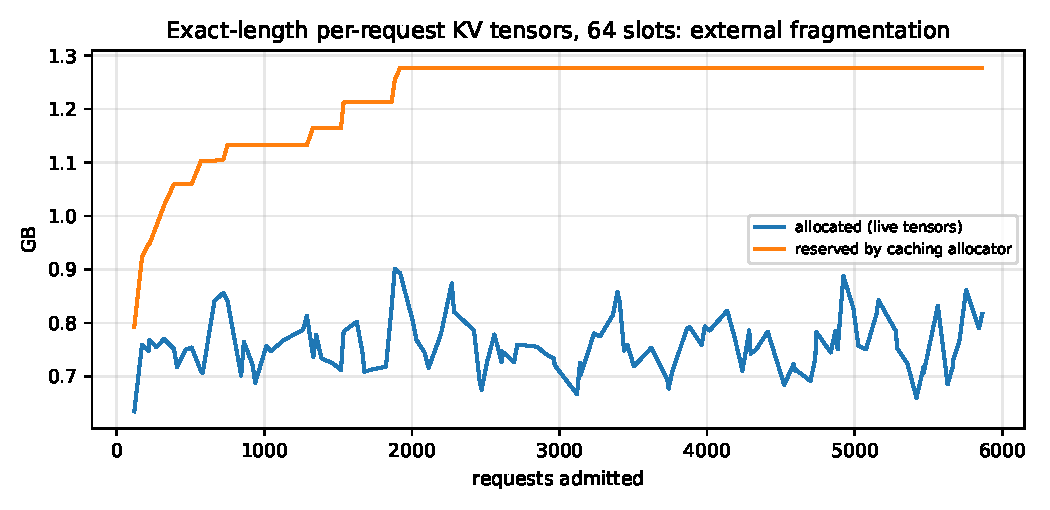
\includegraphics[width=0.75\linewidth]{srv_alloc_churn.pdf}
\caption{按最终长度为每个请求单独分配 KV 张量（64 槽位、6000 个请求）时，PyTorch 缓存分配器 reserved 与 allocated 的比值。}
\label{fig:churn}
\end{figure}
\Cref{fig:churn} 测的是 lab 没有建模的\emph{外部碎片}：64 个槽位持续为 6000 个请求按最终长度分配、释放 KV 张量。PyTorch 缓存分配器 reserved/allocated 平均 1.68、最大 1.94，
共 57 个段，137 MB 处于“已切分但空闲”状态；也就是说，即使内部碎片为零，变长分配也会让约 40\% 的已保留显存不可用（这些空洞对下一个更长的请求可能太小）。
分页方案一次性分配一个定长池，块大小相同，任何空闲块都能复用，外部碎片为零——这是 PagedAttention 相对“按需 \texttt{torch.empty}”的第二个、常被忽略的收益。

\begin{findingbox}[：KV 显存]
在 4 GiB 预算与 lab 长度分布下，按最大长度预留浪费 86.8\%、只能并发 85 个序列；分页（block=16）浪费 1.26\%、并发 593 个（7.0 倍），与 \texttt{waste.py} 的模型相差 $\le1.2$ 个百分点。
变长张量的反复分配另有约 1.7 倍的 reserved/allocated 外部碎片，定长块池完全消除。
\end{findingbox}

%--------------------------------------------------------------------------
\subsection{GPU B3：真实连续批处理引擎 vs 静态批处理}\label{sec:engine}
负载：300 个请求，长度取 lab 分布（seed 0；平均 prompt 406.1、平均输出 180.8 token），泊松到达 $\lambda\in\{5,10,20,40,80\}$ req/s（seed 1），三种策略共用同一请求序列与 2 GiB KV 池。
SLO 取 TTFT $\le1$ s 且 TPOT $\le50$ ms。所有数据来自 \texttt{engine\_\{static,continuous,chunked\}.jsonl}。

\begin{figure}[H]\centering
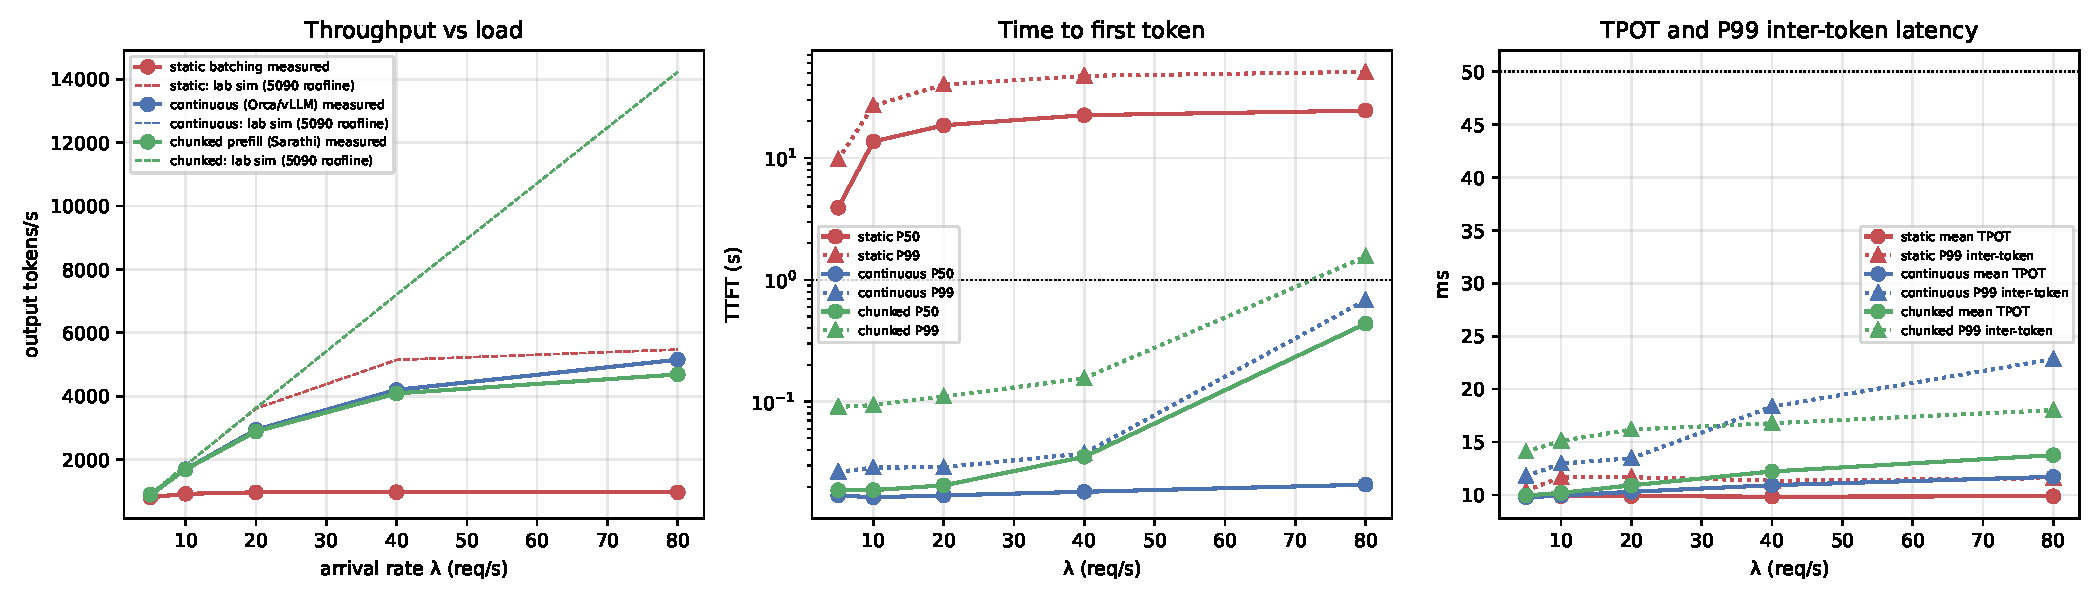
\includegraphics[width=\linewidth]{srv_engine_load.pdf}
\caption{吞吐、TTFT（对数轴）与 TPOT / P99 inter-token 延迟随到达率；虚线为 lab 调度模拟器用实测 5090 参数在同一负载下的预测。}
\label{fig:engload}
\end{figure}

\begin{table}[H]\centering\small
\caption{引擎实测（节选；吞吐为输出 token/s，TTFT 单位 s，TPOT 与 ITL 单位 ms）}
\label{tab:engine}
\begin{tabular}{lrrrrrrrr}
\toprule
策略 & $\lambda$ & tok/s & req/s & TTFT P50 & TTFT P99 & TPOT 均值 & ITL P99 & SLO 达成 \\
\midrule
static & 5 & 811.1 & 4.49 & 3.904 & 9.718 & 9.86 & 10.4 & 7.3\% \\
static & 10 & 921.0 & 5.10 & 13.65 & 26.90 & 9.88 & 11.7 & 2.0\% \\
static & 80 & 968.8 & 5.36 & 24.48 & 51.02 & 9.87 & 11.6 & 0.3\% \\
continuous & 5 & 892.4 & 4.94 & 0.017 & 0.027 & 9.77 & 11.8 & 100\% \\
continuous & 10 & 1696 & 9.38 & 0.016 & 0.029 & 9.94 & 13.0 & 100\% \\
continuous & 40 & 4199 & 23.23 & 0.018 & 0.038 & 10.92 & 18.3 & 100\% \\
continuous & 80 & 5151 & 28.50 & 0.021 & 0.684 & 11.71 & 22.9 & 100\% \\
chunked & 10 & 1694 & 9.37 & 0.019 & 0.094 & 10.19 & 15.1 & 100\% \\
chunked & 40 & 4089 & 22.62 & 0.035 & 0.156 & 12.22 & 16.8 & 100\% \\
chunked & 80 & 4685 & 25.92 & 0.437 & 1.554 & 13.76 & 18.0 & 81.3\% \\
\bottomrule
\end{tabular}
\end{table}

\paragraph{continuous $\gg$ static：命题成立。} 静态批从 $\lambda=10$ 起就饱和在 5.10--5.36 req/s（921--969 tok/s），TTFT 中位数 13.7--24.5 s，SLO 达成率跌到 2\% 以下；
continuous 在 $\lambda=40$ 时仍跟得上到达（23.2 req/s，TTFT P99 38 ms），到 $\lambda=80$ 时 TTFT P99 才升到 0.68 s。所以 continuous 的容量在 40--80 req/s 之间，是 static 的 7.5--15 倍。
注意 $\lambda\ge40$ 时表中 continuous 的“吞吐”被有限请求数压低：最长的请求有约 1000 个输出 token，按约 10 ms/步需要约 10 s 才能结束，
$\lambda=80$ 的 makespan 10.5 s 基本就是这条长尾，所以 5151 tok/s 是容量的下界，不是饱和值。
static 的瓶颈可以直接算出来（\cref{sec:theory-srv}）：每批 42 个请求要陪跑到批内最长输出（期望 723 token）并左填充到批内最长 prompt（期望 2276 token）。

\paragraph{static 的 TPOT 反而最好。} static 的 TPOT 均值 9.86 ms、ITL P99 只有 10.4--11.7 ms，因为批中途不进新请求，decode 从不被 prefill 打断。
它把所有代价都推到了排队上（TTFT 以秒计）——这提醒我们只看 TPOT 会得出错误结论。

\begin{figure}[H]\centering
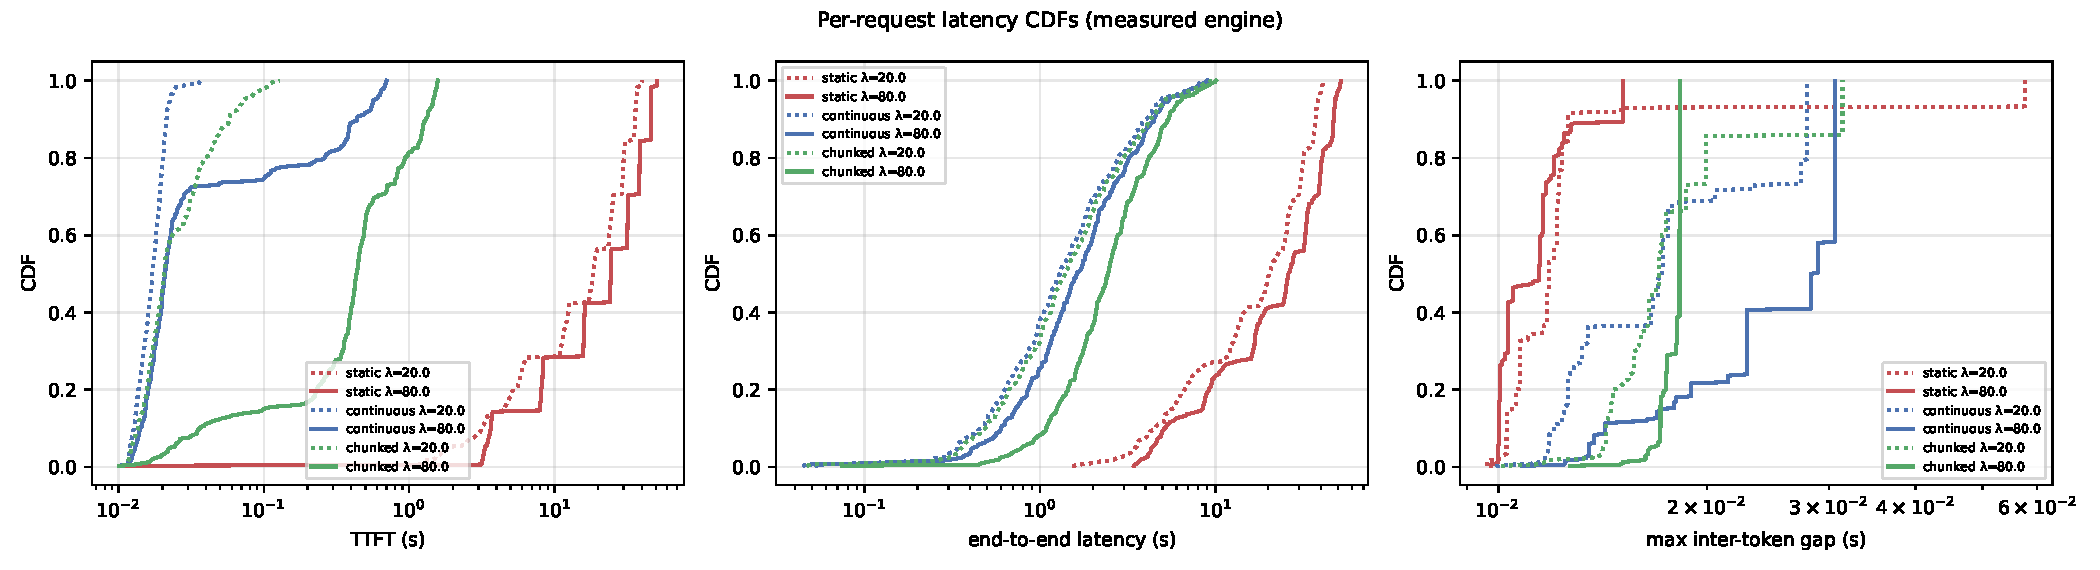
\includegraphics[width=\linewidth]{srv_engine_cdf.pdf}
\caption{逐请求的 TTFT、端到端延迟与最大 inter-token 间隔 CDF（虚线 $\lambda=20$，实线 $\lambda=80$）。}
\label{fig:engcdf}
\end{figure}
\Cref{fig:engcdf}：$\lambda=80$ 时 continuous 约 70\% 的请求 TTFT 在 30 ms 以内，其余在排队中等待 KV 与批位（max\_num\_seqs=128）；
chunked 的 TTFT 整体右移，因为每次迭代只给 prefill 留下 512 token 预算减去 decode 数。右图的阶梯来自每次迭代的离散时间：
最大 inter-token 间隔几乎总是“某一步混入了 prefill”，continuous 下这一步最长 30.6 ms，chunked 下 18.3 ms。

\begin{figure}[H]\centering
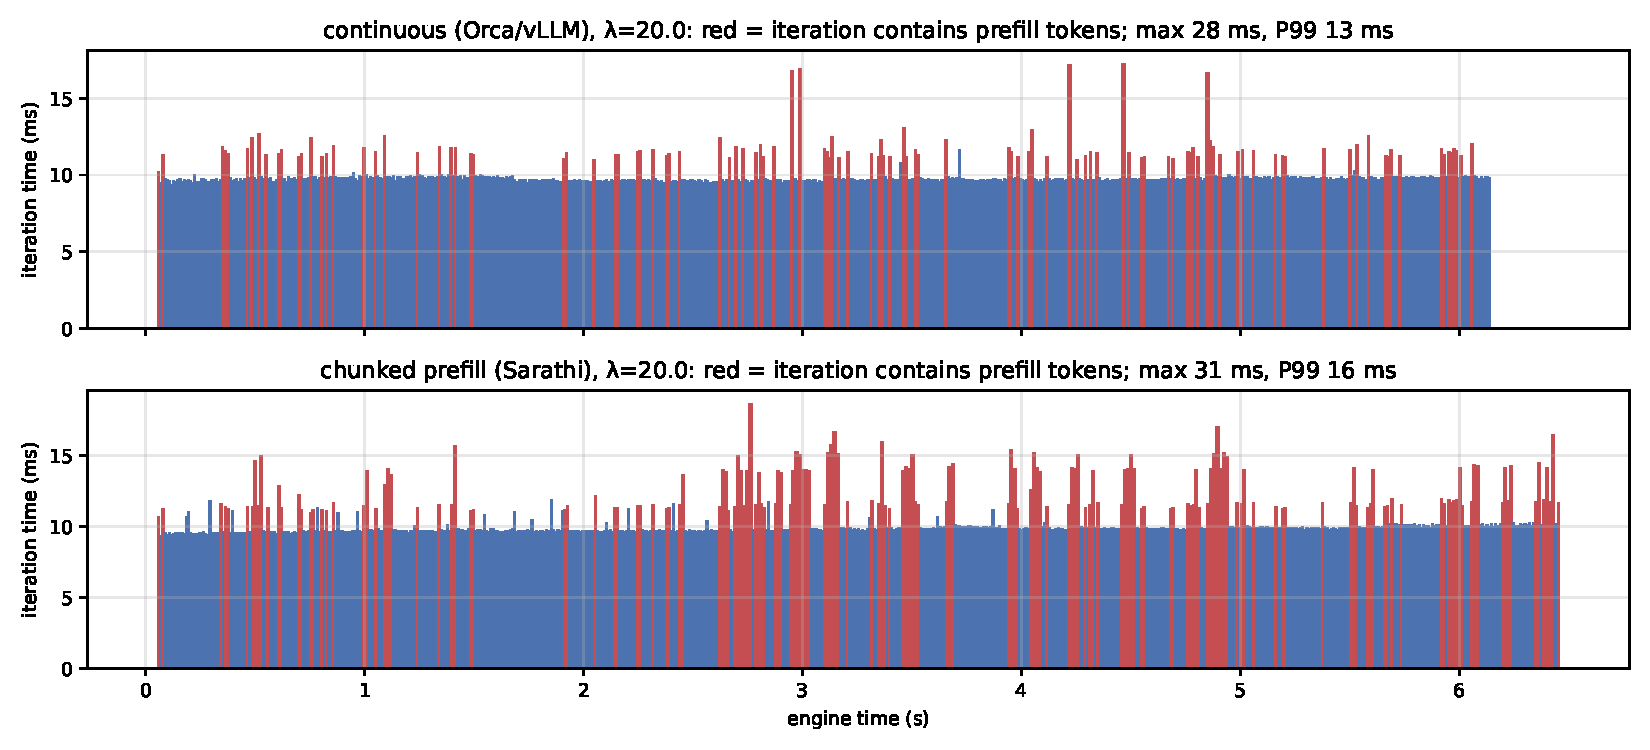
\includegraphics[width=\linewidth]{srv_engine_timeline.pdf}
\caption{$\lambda=20$ 时每次迭代的时间（红色 = 本次迭代含 prefill token）。}
\label{fig:engtl}
\end{figure}
\Cref{fig:engtl}：纯 decode 迭代约 9.8 ms（eager 下发的平台，与 \cref{tab:decode} 的 eager 数一致），含 prefill 的迭代在 continuous 下是孤立的尖峰（最长 27.9 ms），
在 chunked 下是成串的 12--17 ms 小台阶。在 lab 长度分布下（prompt 中位数 256），一次整段 prefill 只比 decode 步多十几 ms，所以 generation stall 并不严重：
$\lambda=20$ 时 continuous 的 ITL P99 为 13.5 ms，chunked 为 16.2 ms——chunked 反而更差，因为它把一个 prompt 拆成多步，每步都要付一次“读已缓存前缀”的代价。

\paragraph{chunked prefill 在长 prompt 下才显出价值。} 为检验 Sarathi 的命题，我们把 10\% 的 prompt 换成 3072 token（\texttt{--long-frac 0.1}，其余不变）：
\begin{figure}[H]\centering
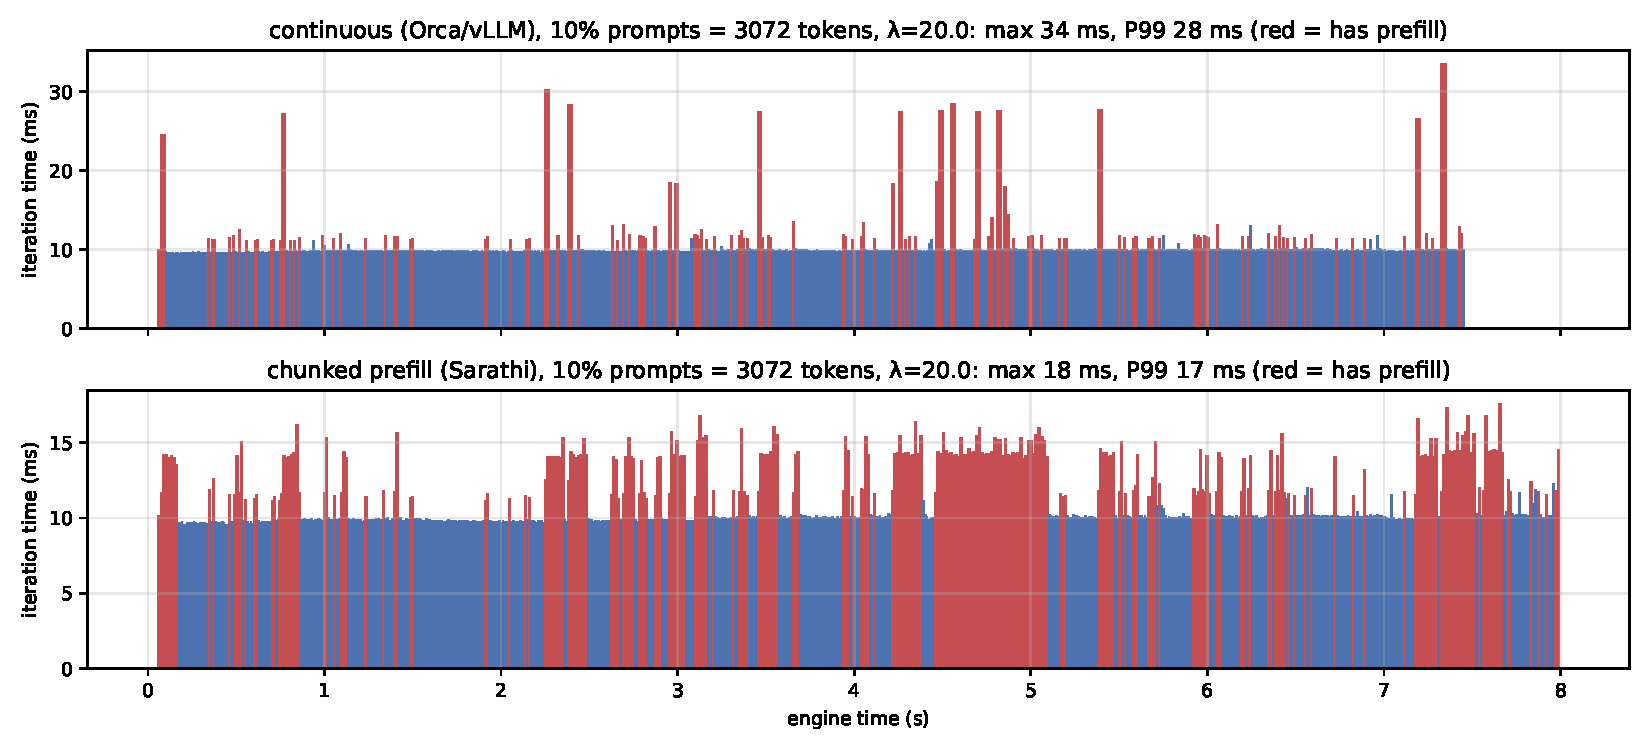
\includegraphics[width=\linewidth]{srv_stall_timeline.pdf}
\caption{10\% prompt 为 3072 token、$\lambda=20$：continuous 的长 prefill 造成 25--34 ms 的尖峰（所有在跑的 decode 都被卡住），chunked 把每步限制在 18 ms 以内。}
\label{fig:stalltl}
\end{figure}
\begin{figure}[H]\centering
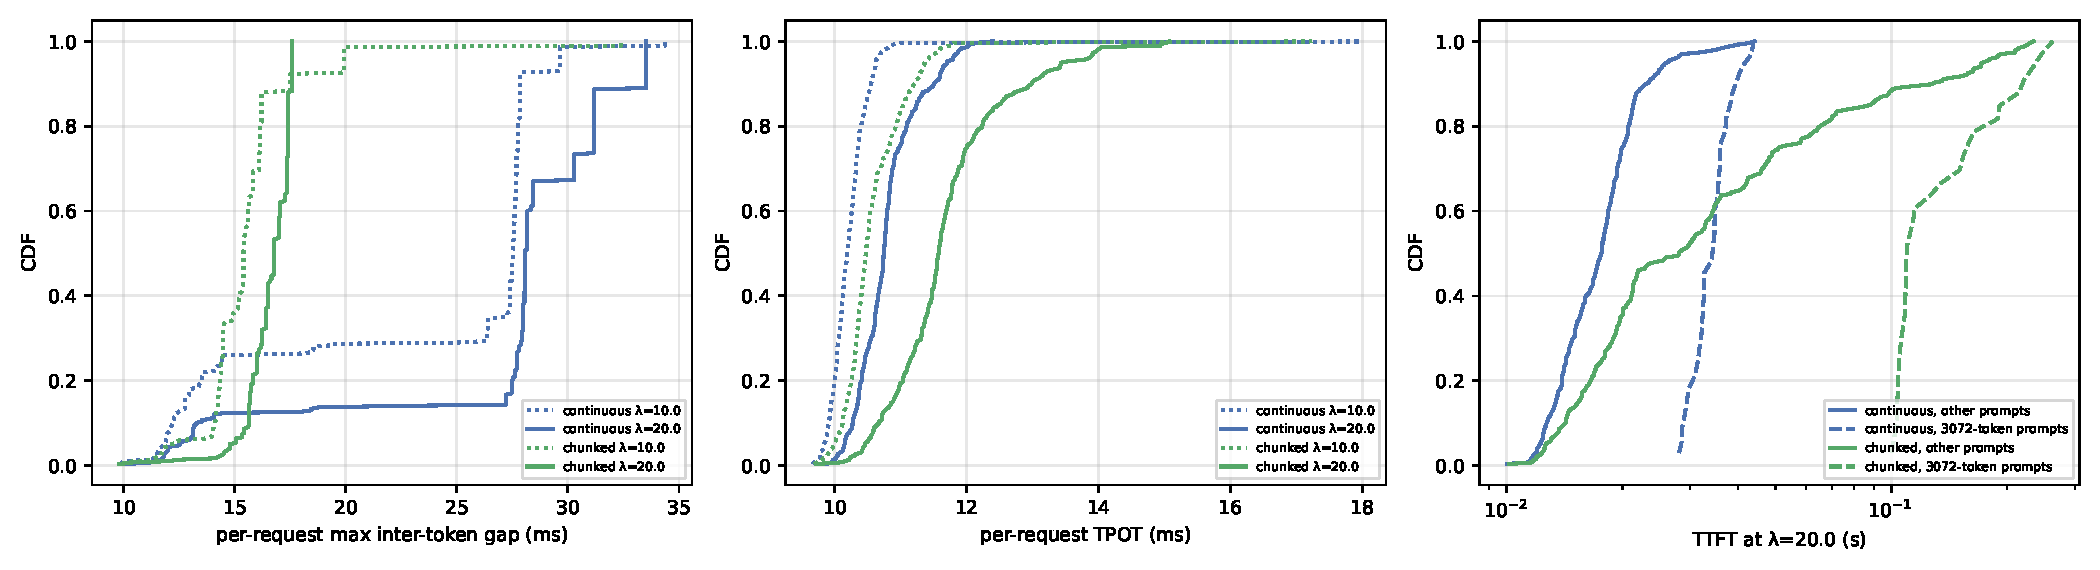
\includegraphics[width=\linewidth]{srv_stall_cdf.pdf}
\caption{同一负载下：逐请求的最大 inter-token 间隔、TPOT，以及 $\lambda=20$ 时长/短 prompt 的 TTFT。}
\label{fig:stallcdf}
\end{figure}
\begin{table}[H]\centering\small
\caption{长 prompt 负载（10\% 为 3072 token，$\lambda=20$；\texttt{engine\_*\_long.jsonl}）}
\label{tab:stall}
\begin{tabular}{lrr}
\toprule
指标 & continuous & chunked (512) \\
\midrule
最长迭代 / P99 迭代 (ms) & 33.5 / 27.9 & 17.6 / 16.5 \\
逐请求最大 ITL：P50 / P99 (ms) & 28.1 / 33.5 & 16.8 / 17.6 \\
TPOT 均值 / P99 (ms) & 10.79 / 12.02 & 11.71 / 14.94 \\
TTFT P50：3072-token prompt / 其他 (s) & 0.034 / 0.018 & 0.110 / 0.028 \\
吞吐 (tok/s) & 2909 & 2833 \\
\bottomrule
\end{tabular}
\end{table}
\Cref{fig:stalltl,fig:stallcdf,tab:stall}：continuous 下一半请求至少经历一次 28 ms 的卡顿（3072 token 的 prefill 与 decode 同批），chunked 把它降到 16.8 ms（$-40\%$），P99 从 33.5 降到 17.6 ms（$-47\%$）。
代价与论文描述一致：长 prompt 的 TTFT 从 34 ms 变成 110 ms（3.2 倍，要分 6 步以上），平均 TPOT 增加 8.5\%，吞吐下降 2.6\%。
即：chunked prefill 是把\emph{尾部的 inter-token 延迟}换成\emph{长 prompt 的 TTFT}，而不是提升吞吐。在本文的小模型上 prefill 便宜，stall 只有 3 倍步长；
对 7B 以上模型、或 prompt 上万 token 时，整段 prefill 可达数百 ms，收益会大得多。

\paragraph{一个实现细节决定了 chunked 的成败。} 第一版引擎对“带已缓存前缀的 prefill 块”用布尔掩码调用 SDPA，PyTorch 因此退回未融合的 math 实现。
$\lambda=20$ 时含 $\ge400$ 个 prefill token 的迭代，新 prompt 块平均 11.83 ms，带前缀的块 17.63 ms；换成 \texttt{causal\_lower\_right} 偏置并显式展开 GQA 头后，带前缀的块降到 15.02 ms
（\texttt{engine\_chunked\_maskedsdpa.jsonl} 保留为消融），$\lambda=80$ 的 chunked 吞吐从 4481 提到 4685 tok/s，ITL P99 从 20.6 降到 18.0 ms。
剩余的约 3 ms 来自每层把前缀页 gather 成连续张量；生产系统（vLLM 的 paged prefill / FlashAttention~\cite{dao2022} varlen + block table）直接在块表上做 prefill attention，没有这一步。

\begin{figure}[H]\centering
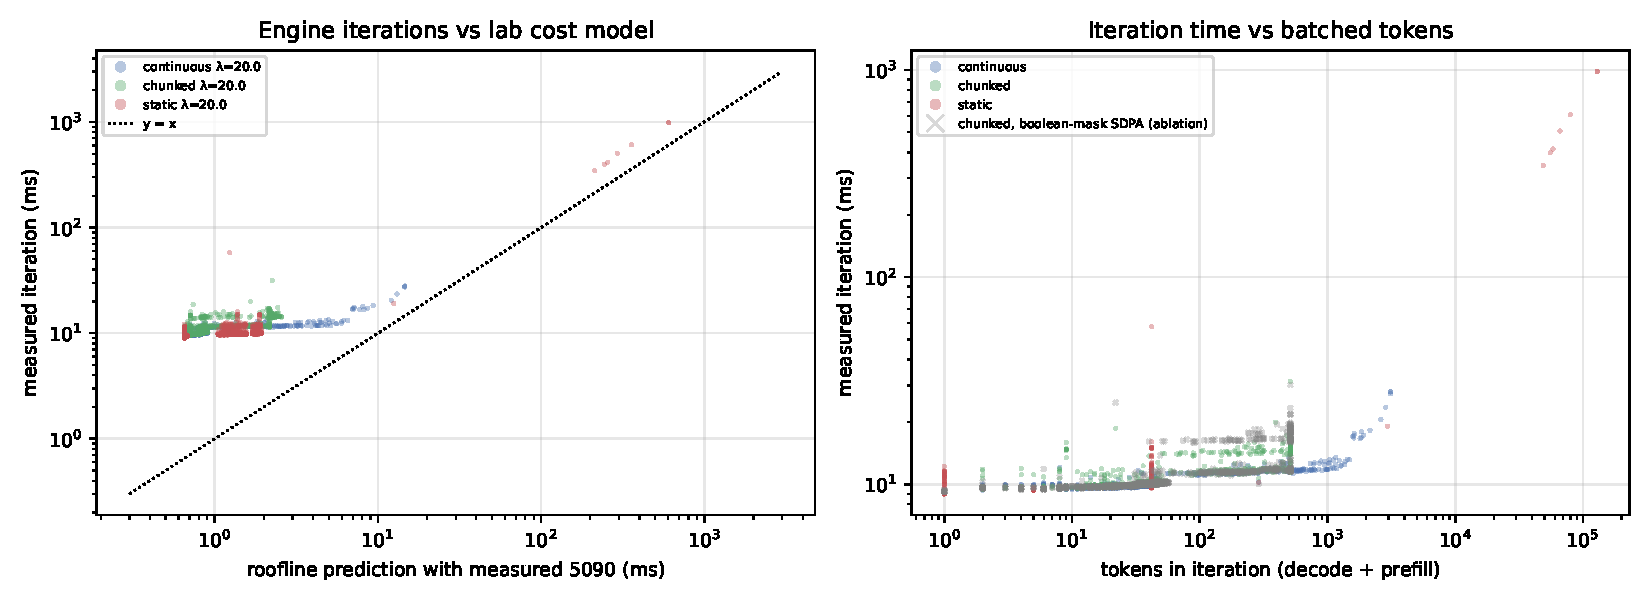
\includegraphics[width=\linewidth]{srv_engine_costmodel.pdf}
\caption{左：每次迭代的实测时间 vs lab 成本模型（实测 5090 参数的 roofline）；右：迭代时间 vs 本次迭代的 token 数（灰叉为布尔掩码版 chunked）。}
\label{fig:engcost}
\end{figure}
\Cref{fig:engcost} 把引擎与 lab 的调度模拟器对上：对 continuous 的 1814 次迭代做线性拟合，实测 $= 9.15\ \text{ms} + 1.03\times$ roofline 预测，
即 roofline 的\emph{斜率}几乎完全正确（GPU 上真正的工作量模型没错），缺的是每次迭代约 9.2 ms 的固定开销（Python 调度 + eager 下发 + 采样同步）。
中位数上实测是模型的 12.2 倍。因此 lab 模拟器用 5090 参数预测 continuous 在 $\lambda=80$ 时 14,235 tok/s、TPOT 0.78 ms，static 30.3 req/s，
都比实测乐观一个数量级；但它对三种策略的\emph{排序}与“static 先饱和”的结论是对的。把固定开销加进 \texttt{CostModel} 是让模拟器可信的最小修改。

\begin{findingbox}[：调度]
真实引擎上 continuous batching 的容量是 static 的 7.5--15 倍（static 饱和于 5.36 req/s，continuous 在 $\lambda=40$ 时 TTFT P99 仍为 38 ms）。
chunked prefill 只有在长 prompt 下才有价值：10\% 为 3072 token 时把逐请求最大卡顿 P99 从 33.5 ms 降到 17.6 ms，代价是长 prompt 的 TTFT 变成 3.2 倍；lab 分布下它反而略差。
lab 成本模型的斜率正确（1.03），缺少约 9 ms/迭代的固定开销。
\end{findingbox}

\subsection{GPU B4：对照 vLLM 0.11（RTX 6000D）}\label{sec:vllm}

\texttt{gpu/vllm\_bench.py} 用同一个 Qwen2.5-0.5B bf16、同样的长度分布与 Poisson 到达（同种子）、同样 2~GiB KV 预算、最多 128 序列、8192 批 token，输出强制到采样长度。
vLLM V1 总是对长 prefill 分块，所以最接近的自写策略是 \texttt{chunked}。两边都在 RTX 6000D 上运行。

\begin{figure}[H]\centering
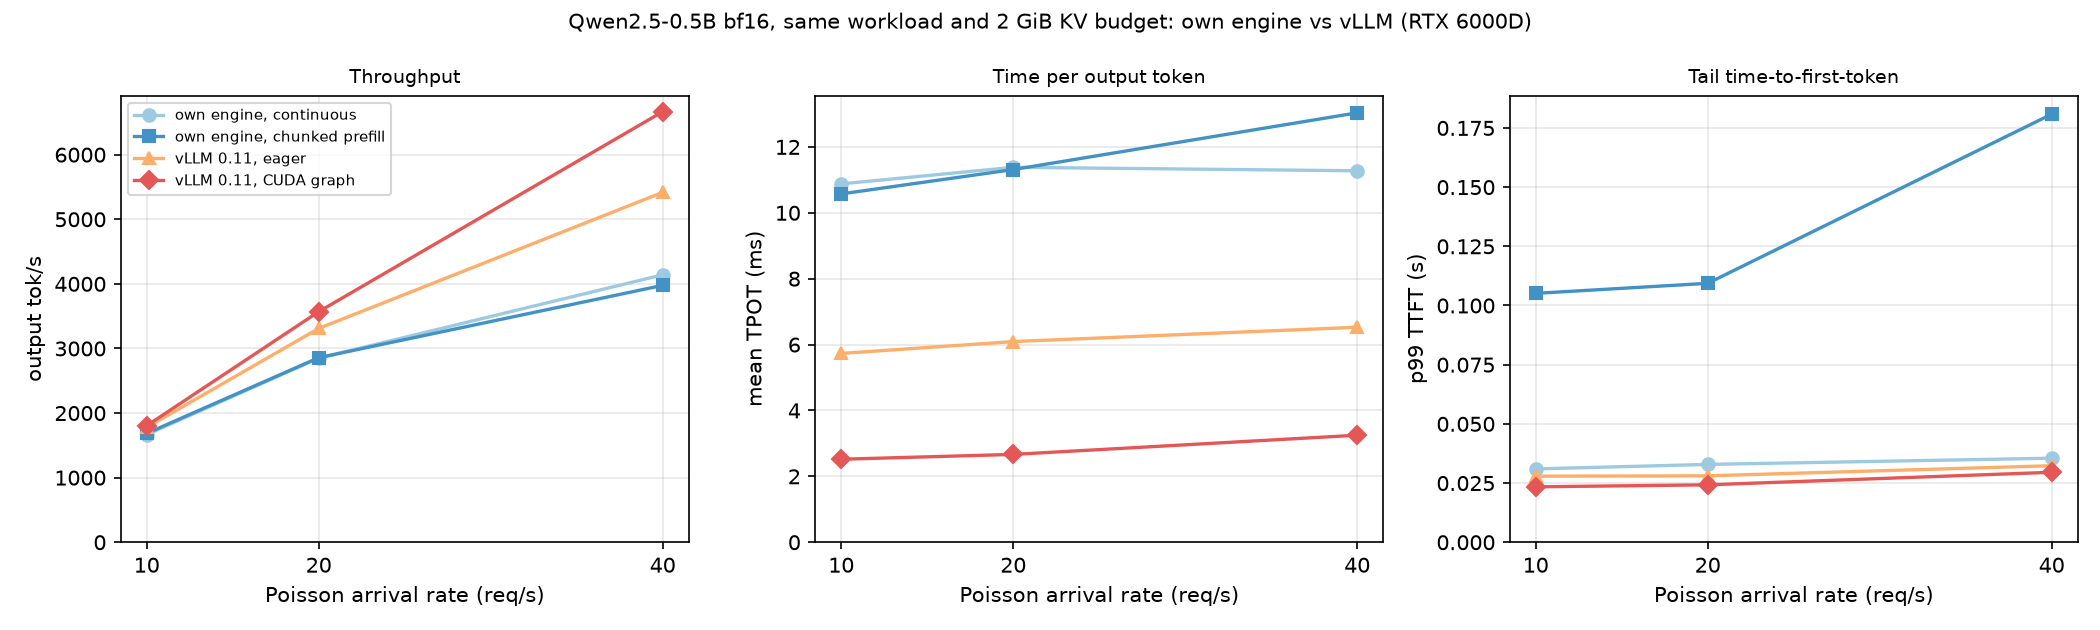
\includegraphics[width=\linewidth]{rtx6000d/vllm_compare.png}
\caption{自写引擎（continuous / chunked）与 vLLM 0.11（eager / CUDA graph）在三个到达率下的吞吐、TPOT 与 TTFT P99。}
\label{fig:vllm}
\end{figure}

\begin{table}[H]\centering\small
\caption{吞吐（tok/s）/ TPOT（\texttt{vllm\_compare.csv}）}\label{tab:vllm}
\begin{tabular}{rllll}
\toprule
$\lambda$（req/s） & 自写 continuous & 自写 chunked & vLLM eager & vLLM CUDA graph \\
\midrule
10 & 1666 / 10.9 ms & 1685 / 10.6 ms & 1778 / 5.7 ms & 1804 / 2.5 ms \\
20 & 2849 / 11.4 ms & 2857 / 11.3 ms & 3310 / 6.1 ms & 3569 / 2.7 ms \\
40 & 4140 / 11.3 ms & 3977 / 13.0 ms & 5417 / 6.5 ms & 6666 / 3.2 ms \\
\bottomrule
\end{tabular}
\end{table}

\begin{itemize}
  \item $\lambda=10$ 时吞吐差不多（1666 对 1804）：负载没压满，大家都在服务到达的请求；差别全在每 token 延迟，TPOT 10.9 对 2.5 ms，4.3 倍。
  \item $\lambda=40$ 时 vLLM 吞吐是 1.61 倍：每步更快，同样到达率下排队更少、批更满。
  \item 尾 TTFT：自写 chunked 在 $\lambda=40$ 时 P99 181 ms，vLLM 30 ms；vLLM 的分块预算与调度顺序让新请求更快拿到首 token，自写版本的块大小没有调。
\end{itemize}

\begin{findingbox}[：8.1 ms 的 TPOT 差拆成两段]
$\lambda=40$ 时 vLLM eager 6.5 ms，自写 11.3 ms：约 5 ms 是 Python 调度与逐 kernel 下发的差（即 \cref{fig:engcost} 里每迭代 9.15 ms 的固定开销）；
CUDA graph 再省 3.3 ms。0.5B 模型 decode 的瓶颈按顺序是：调度/下发 → kernel 数 → 带宽，与 \cref{sec:roofline} 的结论一致。
\end{findingbox}

\begin{caveatbox}
0.5B 模型、单卡、随机 token 的提示（前缀缓存关闭）；大模型上 GEMM 时间变长，下发开销占比小得多，差距会收窄。
vLLM 0.11 要求 transformers < 5，venv 若继承系统的 transformers 5.x 会在 \texttt{all\_special\_tokens\_extended} 处报错。
\end{caveatbox}

%==========================================================================
\section{与理论模型的对照}\label{sec:theory-srv}

\subsection{decode 步时间与拐点}
lab 的成本模型是纯 roofline：$t = \max(F/P,\ (W + \kappa\sum_i \text{ctx}_i)/\text{BW})$，其中 $W=0.988$ GB（bf16 权重），$\kappa=12{,}288$ B/token。
实测表明还需要一个与 batch 无关的固定项 $t_0$：
\begin{equation}
t(B,\text{ctx}) \approx t_0 + \frac{W + \kappa B\,\text{ctx}}{\text{BW}_{\text{eff}}},\qquad
t_0 \approx \begin{cases} 1.5\ \text{ms} & \text{CUDA graph（约 1000 个 kernel 的最小执行时间）}\\ 7.5\text{--}9\ \text{ms} & \text{eager（加上 Python 下发）}\end{cases}
\end{equation}
令步时间相对 $B=1$ 翻倍，得拐点 $B^\star \approx t(1)\cdot\text{BW}/(\kappa\,\text{ctx}) = 2.16\,\text{ms}\times1.518\,\text{TB/s}/(12{,}288\,\text{ctx}) \approx 266{,}846/\text{ctx}$：
ctx = 128/512/2048/8192 时预测 2085/521/130/33，实测 512/256/128/64。ctx=2048 时吻合；短上下文时 KV 项小，实际先撞上的是 $d=896$ 的窄 GEMM 效率（\cref{sec:roofline}），拐点比模型早；
长上下文、小 batch 时分页 kernel 的有效带宽远低于拷贝带宽（\cref{fig:pbw}），所以拐点比模型晚。模型抓住了“拐点 $\propto 1/\text{ctx}$”，但常数要靠实测。

\subsection{分页浪费}
若请求在用长度 $\ell$ 对块大小 $b$ 的余数近似均匀，每序列的尾块浪费期望为 $(b-1)/2$ 个 token，浪费比例
\begin{equation}
w(b) \approx \frac{(b-1)/2}{\bar\ell + (b-1)/2}.
\end{equation}
由实测在用字节反推的平均在用长度 $\bar\ell \approx 581$--$583$ token（例如 block=16：$4{,}236{,}496{,}896/12{,}288/593 = 581.4$），代入得
$w(8,16,32,64) = 0.60\%, 1.27\%, 2.60\%, 5.13\%$，实测 0.59\%, 1.26\%, 2.63\%, 5.14\%。按最大长度预留时 $w = 1-\bar\ell/4096$，代入 $\bar\ell$（$565{,}395{,}456/12{,}288/85=541.3$）得 86.8\%，与实测相同。
这说明“分页浪费 $\approx$ 半个块”在真实分配下精确成立，block 的选择只是浪费（$\propto b$）与块表/kernel 开销（$\propto 1/b$）的折中。

\subsection{排队：Little 定律与静态批的容量}
Little~\cite{little1961} 定律 $L=\lambda W$ 对引擎成立：continuous、$\lambda=20$ 时有效到达率 16.26 req/s、平均端到端 1.865 s，$\lambda W = 30.3$；按迭代时间加权的平均在跑序列数为 30.2。
$\lambda=80$ 时 $\lambda W = 61.8$，在跑 58.8，差值约 3 个就是排队中的请求。静态批的容量可以闭式估计：每批 $B_s=42$ 个请求的时间
\begin{equation}
T_{\text{batch}} \approx t_{\text{prefill}}(B_s\cdot \mathbb{E}[\max p]) + \mathbb{E}[\max o]\cdot t_{\text{dec}},
\end{equation}
从 300 个请求中抽 42 个，$\mathbb{E}[\max o]=723$、$\mathbb{E}[\max p]=2276$；实测 $t_{\text{dec}}=9.85$ ms、填充后 prefill 平均 474.5 ms，得 $T_{\text{batch}}\approx7.6$ s，
容量 $42/7.6 = 5.53$ req/s，实测饱和值 5.36 req/s（差 3\%）。平均输出只有 180.8 token，而批要跑 723 步：static 的有效 batch 利用率约 $180.8/723 = 25\%$，
这就是 Orca 的核心论点——continuous 把这 75\% 的空转换成了新请求。

\subsection{成本模型的修正}
引擎迭代的线性拟合 $t = 9.15\,\text{ms} + 1.03\,t_{\text{roofline}}$ 说明：GPU 端工作量的 roofline 模型基本正确，系统性偏差来自每次迭代固定的 CPU 开销。
对 lab 模拟器，把 \texttt{CostModel.step\_time} 改为 $t_0 + t_{\text{roofline}}$（$t_0$ 取 graph 1.5 ms 或 eager 9 ms）即可让绝对数值落到实测附近；
但所有\emph{相对}结论——static 最早饱和、chunked 用 TTFT 换 TPOT 尾部——在不修正时就已成立，因为 $t_0$ 对三种策略相同。

%==========================================================================
\section{面试专题}

\begin{iqbox}{为什么 LLM decode 是访存受限的？batch 大到多少才变成计算受限？}
每个 decode token 对每个权重做 1 次乘加（2 FLOP），读 2 字节（bf16），算术强度约 $B$ FLOP/B；5090 实测 238.7 TFLOP/s / 1.518 TB/s = 157 FLOP/B，
所以纯权重项的拐点是 $B\approx157$。加上 KV 读（每 token 每步 $12{,}288\cdot\text{ctx}$ 字节，强度不随 $B$ 增大），长上下文时永远到不了计算受限。
实测（graph）步时间翻倍的 batch：ctx=128 时 512、ctx=8192 时 64。
\par\textbf{常见错答}：“decode 是计算受限，所以要更大的 GPU”；或只算权重不算 KV——ctx=8192、B=64 时 KV 读量是权重的 6.5 倍。
\end{iqbox}

\begin{iqbox}{小模型 decode 的步时间能用 $W/\text{BW}$ 估吗？}
不能。0.5B 模型 $W/\text{BW}=0.65$ ms，CUDA graph 实测 2.16 ms，eager 实测约 8.5 ms。每步约 1000 个 kernel，每个 kernel 有 µs 级下限；eager 时还要加上 Python 下发。
这正是 CUDA graph、算子融合、多步调度（一次调度跑多步 decode）的动机。
\par\textbf{常见错答}：“GPU 带宽 1.8 TB/s，0.5B 模型 1 GB，所以 1800 tok/s”——实测 batch 1 graph 只有 462 tok/s，eager 约 120 tok/s。
\end{iqbox}

\begin{iqbox}{PagedAttention 解决的是什么问题？代价是什么？}
解决 KV 的内部碎片（按最大长度预留）与外部碎片（变长张量反复分配释放），浪费上界为每序列一个块尾，期望约 block/2 个 token。
代价是 attention 要按块表间接寻址：本文 Triton kernel 随机物理块与按序物理块的时间差 $<1\%$，所以代价几乎为零——前提是 kernel 原生支持块表，而不是先 gather 再算（慢 2.2--10.7 倍）。
\par\textbf{常见错答}：“分页让 attention 变慢 20--30\%”——那是早期不融合实现的数字；或“分页节省了 KV 计算”——它只省显存（与无效带宽），不省 FLOPs。
\end{iqbox}

\begin{iqbox}{block size 怎么选？}
浪费 $\approx \text{block}/2$ token/序列，占比 $\approx \text{block}/(2\bar L)$；块越小块表越大、kernel 每次加载的连续段越短。本文 kernel 固定每次载 64 token，block 8--64 时间差在 $\pm15\%$ 内，
所以选择由浪费与块表开销决定；vLLM 默认 16。prefix caching 时块越小共享粒度越细。
\par\textbf{常见错答}：“block 越大 kernel 越快，所以选 256”——对本文 kernel 不成立，且浪费线性增大。
\end{iqbox}

\begin{iqbox}{continuous batching 为什么比 static batching 吞吐高这么多？}
static 批里每个序列要陪跑到批内最长输出结束（输出长度右偏，最长常是均值的数倍），还要等凑满一批才开始；continuous 每次迭代把完成的序列换成新请求，批中始终是“活”的 token。
在 decode 拐点之前加 batch 几乎免费，所以有效 batch 越大吞吐越高。本文实测见 \cref{sec:engine}。
\par\textbf{常见错答}：“continuous batching 让单步更快”——单步时间不变甚至更长，提高的是每步的有用 token 数；或忽略它对 KV 管理的依赖：没有分页，动态换入换出会被碎片拖垮。
\end{iqbox}

\begin{iqbox}{chunked prefill 解决什么问题？有什么代价？}
continuous batching 把整段长 prompt 与 decode 放进同一次迭代，那一步的时间由 prefill 决定，所有在跑的 decode 都被卡住（generation stall），表现为 TPOT 的长尾与 max inter-token latency。
chunked prefill 给每次迭代一个 token 预算（本文 512），先放 decode 再切 prefill，使每步时间有界。代价：长 prompt 的 TTFT 变长（要分多步），每块要重复读已缓存的 KV；
本文实测 512 token 的 prefill 只有 57.1 TFLOP/s，块太小会降低 prefill 效率。
\par\textbf{常见错答}：“chunked prefill 提高吞吐”——它主要改善尾延迟与 SLO 达成率，吞吐通常持平或略降。
\end{iqbox}

\begin{iqbox}{TTFT 和 TPOT 分别由什么决定？怎么权衡？}
TTFT = 排队 + prefill（若被切块，还包括与 decode 混跑的若干步）；TPOT = decode 步时间，受同批 prefill 干扰。优先 prefill（vLLM v0 默认）利于 TTFT、伤 TPOT；
优先 decode + 切块（Sarathi）利于 TPOT、伤长 prompt 的 TTFT。彻底分离的方案是 prefill/decode 分离部署（DistServe~\cite{zhong2024}、Splitwise~\cite{patel2024}）。
\par\textbf{常见错答}：只看平均吞吐；或把 TPOT 定义成 e2e/输出长度（含了 TTFT，会掩盖 decode 卡顿）。
\end{iqbox}

\begin{iqbox}{KV 显存不够了怎么办？swap 还是 recompute？}
recompute 丢掉 KV、之后重新 prefill，代价是一次 prefill 的计算（计算受限，约 $2Ns$ FLOP）；swap 把块搬到 CPU，代价是 $12{,}288\cdot s$ 字节过 PCIe（5090 实测 56.5 GB/s）。
短序列 recompute 更便宜，长序列（或 GQA 下 KV 很小）swap 更划算；vLLM 默认 recompute。
\par\textbf{常见错答}：“swap 总是更好，因为不浪费计算”——小 batch 时 GPU 计算是空闲的，recompute 几乎免费，而 swap 占 PCIe 并需要同步。
\end{iqbox}

\begin{iqbox}{给定 GPU 显存，最大并发数怎么估？}
并发 $\approx (\text{显存} - W - \text{激活/工作区}) / (\text{每 token KV}\times\text{平均在用长度}\times(1+\text{浪费率}))$。本文 4 GiB KV、Qwen2.5-0.5B 时，
分页方案的并发数是按最大长度预留的约 8 倍（\cref{sec:waste}）。并发数再受 decode 拐点与 SLO 限制，不是越大越好。
\par\textbf{常见错答}：用最大上下文长度算每序列 KV——那正是 vLLM 之前的系统的做法。
\end{iqbox}

\paragraph{20 秒电梯陈述。}
“我在一张 RTX 5090 上从权重文件开始写了一个小型推理引擎：自写 Qwen2.5-0.5B 前向（fp32 下与 HF 的 logits 差 $1.5\times10^{-4}$），
Triton 分页 decode attention（间接寻址开销 $<1\%$，比 gather 快 2--10 倍），以及分页 KV + iteration-level 调度 + chunked prefill 的服务循环。
实测发现：小模型 decode 的瓶颈不是 HBM 而是 kernel 数和 CPU 下发，roofline 低估 3 倍；分页把 KV 浪费从八成以上降到个位数百分比；continuous batching 相对 static 的吞吐优势在真实 GPU 上同样成立。”

\paragraph{STAR 故事：一个“偏小”的浪费率。}
\textbf{S}：第一次在 GPU 上测分页 KV 的浪费时，我按“均匀抽请求、均匀抽时刻”做快照，得到的浪费数字和 lab 的 \texttt{waste.py} 对不上。
\textbf{T}：要确定是 GPU 实现有 bug，还是测量方法与模型的定义不一致。
\textbf{A}：回到定义：\texttt{waste.py} 是\emph{生命周期时间平均}，长输出请求在系统里驻留更久，在稳态快照中出现的概率应正比于输出长度。
均匀抽请求等于给短请求过多权重。我把采样改成按输出长度的 size-biased 抽样，并在 CPU 上先验证新采样下的期望与 \texttt{waste.py} 一致，再上 GPU 重测。
\textbf{R}：实测与模型对齐（\cref{tab:waste}）。教训：任何“快照”统计都要先问是按事件平均还是按时间平均（检查悖论，inspection paradox）；Little 定律 $L=\lambda W$ 也是同一回事。

%==========================================================================
\section{局限与注意事项}\label{sec:caveat}
\begin{caveatbox}
\begin{itemize}
\item \textbf{共享 GPU}：7 个代理共用一张卡，所有 GPU 命令在文件锁下串行，但同一时刻不会有两个任务同时用 GPU；计时仍可能受时钟频率与热状态影响，单次运行未做多次重复。
\item \textbf{2 个 CPU 核}：eager 下发受限的结论（8.5 ms/步）依赖 CPU；在 16 核服务器上 eager 时间会更短，但“graph 2.16 ms 仍比 roofline 慢 3.3 倍”与 CPU 无关。
\item \textbf{引擎用 eager}：引擎每次迭代的批形状都不同，没有用 CUDA graph，所以引擎的步时间约为 graph 的 3--4 倍；绝对吞吐因此偏低，但三种策略在同一条件下比较。
\item \textbf{虚拟时钟}：引擎按实测迭代 wall time 推进时钟、空闲时跳到下一个到达，不真实 sleep；这等价于“到达过程与 GPU 时间解耦”的离散事件仿真，但忽略了网络与 tokenizer 开销。
\item \textbf{静态批的左填充未加掩码}：只用于计算成本（step 时间与显存），生成的 token 不保证与无填充时一致；正确性测试只比较批中最长 prompt 的序列。
\item \textbf{合成请求}：prompt 为随机 token，输出长度预先采样并强制生成到该长度（忽略 EOS），与 lab 模拟器一致；真实分布的长尾可能更重。
\item \textbf{单一模型}：只测了 0.5B；7B 级模型的 decode 会更接近带宽 roofline（单层权重更大、kernel 数相同），roofline 偏差会小得多。
\item \textbf{bf16 与 HF 的对齐}：bf16 下与 HF 的 logits 最大差 1.22、argmax 一致率 95.8\%，原因是融合 GEMM 与 HF 分开计算的舍入顺序不同；fp32 下完全对齐，说明实现正确。
\end{itemize}
\end{caveatbox}

%==========================================================================
\section{结论}
\begin{enumerate}
\item \textbf{roofline 只描述最后一层瓶颈。} Qwen2.5-0.5B 的 decode 在 eager 下每步约 8.5 ms（CPU 下发），CUDA graph 下 2.16 ms（kernel 数），带宽 roofline 0.65 ms；
拐点 $\propto1/\text{ctx}$（实测 512/256/128/64），但常数要实测。prefill 在 $\gtrsim$2k token 时计算受限，8192 token 达 173.9 TFLOP/s。
\item \textbf{分页 attention 的间接寻址几乎免费}（随机物理块 vs 按序 $<1\%$），前提是 kernel 原生读块表；gather 再算慢 2.2--10.7 倍，预留 4096 的 SDPA 慢 3.3--6.9 倍。
\item \textbf{KV 浪费的模型在真实分配下精确成立}：最大长度预留 86.8\%（并发 85），分页 block=16 为 1.26\%（并发 593，7.0 倍），与 \texttt{waste.py} 差 $\le1.2$ 个百分点，
分页浪费 $\approx(b-1)/2$ token/序列；另有 lab 未建模的外部碎片（reserved/allocated 平均 1.68），定长块池消除之。
\item \textbf{continuous batching 的容量是 static 的 7.5--15 倍}；static 饱和于 5.36 req/s，与闭式容量模型（5.53）差 3\%，有效 batch 利用率仅约 25\%。
\item \textbf{chunked prefill 用长 prompt 的 TTFT 换 decode 尾延迟}：10\% prompt 为 3072 token 时最大卡顿 P99 33.5$\to$17.6 ms，长 prompt TTFT 3.2 倍、吞吐 $-2.6\%$；
lab 分布（短 prompt）下无收益。其效果还强依赖于“带前缀的 prefill 块”的 attention 实现（布尔掩码 SDPA 每块多 5.8 ms）。
\item \textbf{lab 成本模型斜率对、截距错}：引擎迭代 $=9.15$ ms $+1.03\times$roofline；加入固定开销项即可修正绝对数值，相对结论不变。
\end{enumerate}

\begin{thebibliography}{99}
\bibitem{kwon2023} W.~Kwon et al. Efficient Memory Management for Large Language Model Serving with PagedAttention. SOSP 2023.
\bibitem{yu2022} G.-I.~Yu et al. Orca: A Distributed Serving System for Transformer-Based Generative Models. OSDI 2022.
\bibitem{agrawal2024} A.~Agrawal et al. Taming Throughput-Latency Tradeoff in LLM Inference with Sarathi-Serve. OSDI 2024.
\bibitem{williams2009} S.~Williams, A.~Waterman, D.~Patterson. Roofline: An Insightful Visual Performance Model for Multicore Architectures. CACM 2009.
\bibitem{pope2023} R.~Pope et al. Efficiently Scaling Transformer Inference. MLSys 2023.
\bibitem{dao2022} T.~Dao et al. FlashAttention: Fast and Memory-Efficient Exact Attention with IO-Awareness. NeurIPS 2022.
\bibitem{zhong2024} Y.~Zhong et al. DistServe: Disaggregating Prefill and Decoding for Goodput-optimized Large Language Model Serving. OSDI 2024.
\bibitem{patel2024} P.~Patel et al. Splitwise: Efficient Generative LLM Inference Using Phase Splitting. ISCA 2024.
\bibitem{little1961} J.~D.~C.~Little. A Proof for the Queuing Formula $L=\lambda W$. Operations Research 1961.
\bibitem{tillet2019} P.~Tillet, H.~T.~Kung, D.~Cox. Triton: An Intermediate Language and Compiler for Tiled Neural Network Computations. MAPL 2019.
\end{thebibliography}

\end{document}
